%%%%%%%%%%%%%%%%%%%%%%%%%%%%%%%%%%%%%%%%%%%%%%%%%%%%%%%%%%%%
%%% LIVECOMS ARTICLE TEMPLATE FOR BEST PRACTICES GUIDE
%%% ADAPTED FROM ELIFE ARTICLE TEMPLATE (8/10/2017)
%%%%%%%%%%%%%%%%%%%%%%%%%%%%%%%%%%%%%%%%%%%%%%%%%%%%%%%%%%%%
%%% PREAMBLE
\documentclass[9pt,tutorial]{livecoms}
% Use the 'onehalfspacing' option for 1.5 line spacing
% Use the 'doublespacing' option for 2.0 line spacing
% Use the 'lineno' option for adding line numbers.
% Use the "ASAPversion' option following article acceptance to add the DOI and relevant dates to the document footer.
% Use the 'pubversion' option for adding the citation and publication information to the document footer, when the LiveCoMS issue is finalized.
% The 'bestpractices' option for indicates that this is a best practices guide.
% Omit the bestpractices option to remove the marking as a LiveCoMS paper.
% Please note that these options may affect formatting.

% NOTES
% when importing references from EndNote, remove the type = {Journal Article}. It messes with the livecoms bibtex style somehow...
% Place a \@ between all-caps words and punctuation ("This is a sentence about GIST\@. This is ...")
% Place a protected space (~) between "Figure" and the reference. The same with tables.

\usepackage{lipsum} % Required to insert dummy text
\usepackage[version=4]{mhchem}
\usepackage{siunitx}
\DeclareSIUnit\Molar{M}
\usepackage[italic,LGRgreek]{mathastext}
\graphicspath{{figures/}}

\usepackage{listings}
\usepackage{tabularx}

%%%%%%%%%%%%%%%%%%%%%%%%%%%%%%%%%%%%%%%%%%%%%%%%%%%%%%%%%%%%
%%% IMPORTANT USER CONFIGURATION
%%%%%%%%%%%%%%%%%%%%%%%%%%%%%%%%%%%%%%%%%%%%%%%%%%%%%%%%%%%%

\newcommand{\versionnumber}{1.0}  % you should update the minor version number in preprints and major version number of submissions.
\newcommand{\githubrepository}{\url{https://github.com/liedllab/gist-tutorial}}  %this should be the main github repository for this article

%%%%%%%%%%%%%%%%%%%%%%%%%%%%%%%%%%%%%%%%%%%%%%%%%%%%%%%%%%%%
%%% ARTICLE SETUP
%%%%%%%%%%%%%%%%%%%%%%%%%%%%%%%%%%%%%%%%%%%%%%%%%%%%%%%%%%%%
\title{Quantifying Spatially Resolved Hydration Thermodynamics Using Grid Inhomogeneous Solvation Theory [Article v\versionnumber]}

\author[1\authfn{1}]{Franz Waibl}
\author[1\authfn{1}]{Valentin J Hoerschinger}
\author[2]{Vjay Molino}
\author[1]{Monica L Fern{\'a}ndez-Quintero}
%\author[1,2]{Firstname Middlename Familyname}
%\author[2]{Firstname Initials Surname}
\author[4]{Daniel R Roe}
\author[1*]{Klaus R Liedl}
\author[2*]{Michael K Gilson}
\author[2*]{Tom Kurtzman}
\affil[1]{Department of General, Inorganic and Theoretical Chemistry, University of Innsbruck, Austria}
\affil[2]{Institution 2}

\corr{email1@example.com}{FMS}  % Correspondence emails.  FMS and FS are the appropriate authors initials.
\corr{email2@example.com}{FS}

\orcid{Author 1 name}{AAAA-BBBB-CCCC-DDDD}
\orcid{Author 2 name}{EEEE-FFFF-GGGG-HHHH}

\contrib[\authfn{1}]{These authors contributed equally to this work}
%\contrib[\authfn{2}]{These authors also contributed equally to this work}

%\presentadd[\authfn{3}]{Department of General, Inorganic and Theoretical Chemistry, University of Innsbruck, Austria}
%\presentadd[\authfn{4}]{Department, Institute, Country}

\blurb{This LiveCoMS document is maintained online on GitHub at \githubrepository; to provide feedback, suggestions, or help improve it, please visit the GitHub repository and participate via the issue tracker.}

%%%%%%%%%%%%%%%%%%%%%%%%%%%%%%%%%%%%%%%%%%%%%%%%%%%%%%%%%%%%
%%% PUBLICATION INFORMATION
%%% Fill out these parameters when available
%%% These are used when the "pubversion" option is invoked
%%%%%%%%%%%%%%%%%%%%%%%%%%%%%%%%%%%%%%%%%%%%%%%%%%%%%%%%%%%%
\pubDOI{10.XXXX/YYYYYYY}
\pubvolume{<volume>}
\pubissue{<issue>}
\pubyear{<year>}
\articlenum{<number>}
\datereceived{Day Month Year}
\dateaccepted{Day Month Year}


%%% Shortcuts and macros
\newcommand{\dgsolv}{\Delta G_\textup{solv}}
\newcommand{\software}{\texttt}
\newcommand{\todo}{\textcolor{red}}
\newcommand\inlinecode{\texttt}

% The \neq command looks messy by default. Replace it by our own makeshift version.
\renewcommand{\neq}{\setbox0\hbox{=}\rlap{\hbox to \wd0{\hss /\hss}}\box0}

\lstset{
	basicstyle=\ttfamily\footnotesize,
	inputencoding=utf8,
	extendedchars=true,
	literate={Å}{{\AA}}1,
	backgroundcolor = \color[rgb]{0.9, 0.9, 0.9},
}
\lstdefinestyle{code}{}
\lstdefinestyle{cpptraj}{title={\centering Cpptraj}}
\lstdefinestyle{bash}{title={\centering Command-line}}
\lstdefinestyle{amber-in}{title={\centering Amber input}}
\lstdefinestyle{pymol}{title={\centering Pymol}}
\lstdefinestyle{python}{
	title={\centering Python},
	language=Python,
	stringstyle=\color[rgb]{1.0, 0, 0},
	commentstyle=\color[rgb]{0, 0, 0.6}
}
\lstset{style=code}

\DeclareSIUnit{\calorie}{cal}
\DeclareSIUnit{\kcalPerMolASqr}{\kilo\calorie\per\mole\per\angstrom\squared}
\DeclareSIUnit{\Molar}{M}

% TODO: delete for final build
\usepackage{pdfcomment}

%%%%%%%%%%%%%%%%%%%%%%%%%%%%%%%%%%%%%%%%%%%%%%%%%%%%%%%%%%%%
%%% ARTICLE START
%%%%%%%%%%%%%%%%%%%%%%%%%%%%%%%%%%%%%%%%%%%%%%%%%%%%%%%%%%%%

\begin{document}

\begin{frontmatter}
\maketitle

\begin{abstract}
Grid inhomogeneous solvation theory (GIST) is a method to compute the free energy of solvation of a compound on a 3-dimensional grid based on molecular dynamics (MD) simulations.
The high spatial resolution of the GIST output, as well as the decomposition into energy and entropy contributions, allow for highly detailed analyses on both proteins and small molecules. However, this versatility also comes with a significant entry barrier for new users.

In this tutorial, we aim to guide the reader through the most common steps involved in a GIST analysis at the example of the streptavidin-biotin complex.
Furthermore, we discuss the theory of GIST with a focus on practical aspects.
We highlight potential pitfalls and show how to avoid technical difficulties.
We assume familiarity with molecular dynamics simulations as well as the AmberTools package.

%This particular document provides a skeleton illustrating key sections for a Tutorial document.
%Please see the sample \texttt{sample-document.tex} in \url{github.com/livecomsjournal/article_templates/templates} for additional information on and examples of using the LiveCoMS LaTeX class.
%Here we also assume familiarity with LaTeX and knowledge of how to include figures, tables, etc.; if you want examples, see the sample just referenced.
%
%In your work, in this particular slot, please provide an abstract of no more than 250 words.
%Your abstract should explain the main contributions of your article, and should not contain any material that is not included in the main text.
%Please note that your abstract, plus the authorship material following it, must not extend beyond the title page or modifications to the LaTeX class will likely be needed.
\end{abstract}

\end{frontmatter}




\section{Introduction}
\todo{ (vah) Sources and better description of all these methods, more literature research, QSAR based methods? better flow }

\todo{IMO, our article looks too dry. We should have something nice (e.g., an illustration of the GIST method) on the 1st or 2nd page -fwa.}
\todo{Potentially relevant: 10.1021/acs.jcim.7b00520 }

Solvation thermodynamics govern any process involving solutes in a solvent.
%Cite "Theory of Simple Liquids"?
%Solutes are constantly interacting with solvents in their environment, necessitating a good description of these interactions for accurate computational predictions. 
The free energy of solvation is defined as the reversible work needed to insert a solute into the solvent \cite{ben-naim-book}.
Especially the interaction with water is of utmost importance, as many biological processes occur in aqueous environment \cite{Privalov2017-water-review}.
It drives real-world effects such as hydrophobic interactions, binding of ligands to a biomolecule, as well as dynamics and folding of proteins.

%The computational calculation of thermodynamical solvation properties is therefore of particular interest and has been tackled by a wide array of methods.
%Quantum mechanical methods provide the most rigorous description of the underlying potential energy surface (PES) but suffer from high computational cost, allowing only the treatment of small systems and few solvent molecules. 
%More recently, QM/MM approaches and potentials based on deep learning \cite{Smith2017-ani} are trying to bridge the gap to computationally less demanding methods while keeping the accuracy of DFT methods.

A wide range of methods have been devised to compute the free energy of hydration.
Data-driven methods such as QSPR or UNIFAC can deliver good results \cite{Borhani2019-qspr,Fredenslund1975-unifac}, but might be limited to molecules that are similar to those in the training set.
Polarizable continuum models (PCMs) \cite{Miertus1981-pcm} such as COSMO \cite{Klamt1993-cosmo} treat the solvent as a homogeneous phase that reacts to the electrostatic potential of the solute \cite{Mennucci2010-pcm}.
%Molecular mechanics based approaches describe the underlying PES through empirically fit force-fields, which reduce the computational demand of these calculations tremendously.
%This allows for the treatment of large biological systems such as proteins in aqueous solution.
Methods such as MM/PBSA or MM/GBSA \cite{Sitkoff1994-pbsa,Kollman2000-mmpbsa} combine an implicit treatment of solvent electrostatics with structural sampling of the solute.
They can quickly provide results for a large number of structures, but can yield inaccurate results when compared to more rigorous explicit solvent methods \cite{Genheden2015-mmpbsa-review}.

On the other hand, explicit solvation methods model the solvent using individual molecules.
They are generally more accurate than implicit methods, but require a statistical sampling of the solvent conformations \cite{Liu2016-md-solubility,Swails2014-cphmd}.
Molecular dynamics (MD) simulations provide an accurate way of modeling solvent packing in confined areas \cite{Haider2016-water-on-surfaces} and general hydrophobic effects \cite{Pratt2016-hydrophobicity}.

The free energy of solvation can be calculated in a statistically rigorous way using alchemical methods \cite{Liu2016-md-solubility,Mobley2009-dgsolv,Mobley2014-freesolv} such as free energy perturbation (FEP) \cite{Zwanzig1954-reweighting} or thermodynamic integration (TI) \cite{Kirkwood1935-ti}.
However, those methods are unable to provide a spatial interpretation of the results.
Furthermore, splitting the free energy into enthalpy and entropy contributions is challenging \cite{Peter2004-alchemical-entropy}.
%Assuming sufficient sampling, they can accurately predict the free energy of solvation in the boundaries of the assumptions underlying their forcefield. 
%However, the seperation of enthalpic and entropic contributions to the free energy of solvation is difficult with these methods and localizing these contributions not easily possible.

Methods derived from statistical mechanics bridge this gap by providing three-dimensional resolution.
Two major flavors of methods in this group are those based on inhomogeneous fluid solvation theory (IST) \cite{Lazaridis1998} and those based on the Ornstein--Zernike (OZ) equation \cite{Hansen2013-simple-liquids}.
The most important example of OZ-based methods is the reference interaction site model (RISM) \cite{Chandler1972-rism} as well as its extension to three dimensions (3D-RISM) \cite{Kovalenko1998-3drism}.
Those methods compute the atomic solvent distributions by self-consistently solving the OZ integral equation to predict solvation thermodynamics.
%The 3D-RISM approach allows for a decomposition into entropic and enthalpic terms as well as a full localization of the underlying distributions to the solute structure.

On the other hand, methods based on IST generally use a molecular solvent distribution obtained from an MD simulation to compute the free energy of hydration from its enthalpic and entropic contributions.
Examples of those methods include grid inhomogeneous solvation theory (GIST) \cite{Nguyen2012,Ramsey2016}, WaterMap \cite{Young2007-watermap,Abel2008-watermap}, SSTMap \cite{Haider2018-sstmap}, STOW \cite{Li2012-stow} and Solvaware \cite{Huggins2016-solvaware}.
The main limitation of those methods is that they rely on an infinite expansion of the entropy in terms of the density distribution, which is truncated after the first or, sometimes, the second \cite{Nguyen2016-gist-second-order,Waibl2022-gist-solvents} term.
Nevertheless, they have been applied on a wide variety of problems involving both small molecules and biological systems.

In this tutorial, we aim to give the reader an introduction into GIST and its application to calculate solution thermodynamics properties of interest. 

GIST is based on IST, solving the integral equations on a grid. 
This approach is more general than other IST-based methods because it accounts for all solvent regions rather than focusing on high-occupancy solvation sites.
%By simulating the dynamics of a solvent around the solute, GIST calculates thermodynamic properties for a standard solvation process as described by Ben-Naim \cite{ben-naim-book}.
It estimates the solvent density from an MD trajectory and allows for a full localization of entropic and enthalpic contributions on the grid around the solute.
For small molecules, GIST has been shown to reach comparable accuracy to TI by approximating the higher-order entropies as a fraction of the first-order entropy, using a factor of \SI{-0.4} for water \cite{Chen2021,Waibl2022-gist-solvents}.
%applying a linear correction factor (0.6 for water) to the first-order entropy as follows \cite{Chen2021,Waibl2022-gist-solvents}:
%\begin{equation}
%S^\textit{total} = S^\textit{1st-order} \times f
%\end{equation}

Recently, GIST was implemented on the GPU, tremendously improving the calculation speed, and allowing for the treatment of large biological systems such as proteases or antibodies \cite{Kraml2019-gigist}.
Furthermore, an implementation based on the particle mesh Ewald (PME) \cite{Darden1993-pme} method was presented, which improves the consistency between GIST and popular molecular dynamics engines. 
Yet further changes allow the inclusion of other rigid solvents than water \cite{Kraml2020,Waibl2022-gist-solvents} or 
allow for the treatment of salt-water mixtures as solvents \cite{Waibl2021-gist-salt}.

While previous publications \cite{Ramsey2016} and tutorials\footnote{See \url{http://ambermd.org/tutorials/advanced/tutorial25/}} gave insightful pointers how to setup and run GIST calculations, the post-processing was often treated less rigorously. While building on these tutorials, we provide an updated guide to calculating solvation properties using GIST to address recent improvements.
Furthermore, we aim to establish a template for the analysis and interpretation of GIST calculations.

%Here you would explain what problem you are tackling and briefly motivate your work.
%
%In this particular template, we have removed most of the usage examples which occur in \texttt{sample-document.tex} to provide a minimal template you can modify; however, we retain a couple of examples illustrating more unusual features of our templates/article class, such as the checklists, and information on algorithms and pseudocode.
%
%Keep in mind, as you prepare your manuscript, that you should plan for a representative image  which will be used to highlight your article on the journal website and publications. Usually, this would be one of your figures, but it must also be uploaded separately upon article submission. We give specific guidelines for this image on the journal website in the section on article submission (see \url{https://livecomsjournal.github.io/authors/policies/index.html#article-submission}).
%
%Additionally, for well-formatted manuscripts, we recommend that you let LaTeX handle figure/table placement for you as much as possible, so please avoid specifying strenuous float instructions like `[h!]` and `[H]` as much as possible.

\subsection{Scope}

This tutorial provides an example of a GIST workflow that can be easily adapted to different systems. 
In addition to a short introduction of the method and the theory behind it, we present an overview of the different implementations of GIST.
We ease the user into basic GIST analysis at the example of biotin.
Building on the basics, we present a more advanced GIST study of the streptavidin-biotin complex, reflecting on many common aspects of GIST studies.
We show how to interpret the three-dimensional contributions of solvation free energy in a binding pocket and around the ligand.
Additionally, we compute the binding contribution of the free energy of solvation, which requires accurate post-processing of the GIST outputs to avoid unfavorable summation of bias.
We believe that this example study covers a wide range of applications.

Furthermore, we discuss several technical aspects and typical pitfalls of GIST analyses, such as the normalization of voxel values and how to deal with double counting of energy contributions. 
Additionally, we provide a Python library (\software{gisttools}) to unify the analysis of GIST data produced by various versions of GIST and make the post-processing of GIST results more accessible.

After completing this tutorial, we expect the reader to be able to run their own GIST study. 

%Tutorials should endeavor to cover the specific task at hand, and also highlight how the steps might need to be modified (or additional care might need to be taken at particular points) to handle more general cases.
%
%The scope of the tutorial, as well as the expected proficiencies / outcomes for researchers who complete the tutorial, should be clearly defined.
%This will often happen in a specific section or subsection in the article itself.

\section{Prerequisites}

%Here you would identify prerequisites/background knowledge that are assumed by your work, as well as any software/license requirements.

\subsection{Background knowledge}
This tutorial is aimed at users with a solid knowledge of molecular dynamics (MD) simulations.
The user should be able to run MD simulations and analyze the resulting trajectories.
Previous experience of GIST is not necessary.
However, we only provide a short summary of the theory behind GIST in section~\ref{sec:theory} at the end of this tutorial.
For more detailed information, we point the reader towards the primary sources.

The presented analyses are run in Python.
While no programming experience is necessary to follow the tutorial, a basic understanding of Python is advantageous to adjust the code towards different requirements and use-cases.

\subsection{Software/system requirements}
%Tutorials should clearly define what system and/or software requirements the researcher will need to complete the tutorial (e.g., VMD version 1.9 or newer, AMBER, etc.). Tutorials requiring specific software packages must provide instructions and files for the referenced version of the software.
The main implementation of GIST is part of the MD analysis software \software{cpptraj} released with AmberTools \cite{amber22}.

A recent version of \software{cpptraj} should be used, such as the one provided in AmberTools22 or a recent installation from GitHub (\url{https://github.com/Amber-MD/cpptraj}).

The closed-source Amber simulation engine is used in this tutorial to run the MD simulations.
If Amber is not available, other MD engines can be used as long as topologies and trajectories can be produced in a format supported by \software{cpptraj}.
If using GROMACS \cite{Abraham2015-gromacs,Pronk2013-gromacs}, we propose to prepare the topology with AmberTools and convert it using \software{acpype.py} \cite{Sousa_da_Silva2012-acpype}.
%We should actually test that!
Also note that compressed trajectory formats such as \inlinecode{xtc} might bias the entropy calculation due to the loss of precision for the atom positions. \todo{This might be in the technical part}

Furthermore, a recent Python version (>3.6) should be available with the following packages installed:
\begin{itemize}
	\item \software{gisttools} (\url{https://github.com/liedllab/gisttools})
	\item \software{mdtraj (\url{https://www.mdtraj.org/}) \cite{McGibbon2015-mdtraj}}
\end{itemize}

We also show examples using the \software{gistpp} program, which can be obtained from \url{https://github.com/KurtzmanLab/Gist-Post-Processing} (code and documentation).

If the reader prefers to skip the MD and GIST calculation, we also provide the GIST output files with this tutorial, such that the post-processing can be done without any expensive calculations.
We additionally provide a Jupyter notebook \cite{Kluyver2016-jupyter,Granger2021-jupyter} with the presented analyses. 
%We recommend JupyterLab to work with the notebook. Jupyter is available at \url{https://jupyter.org/}.

For the visualization of three-dimensional contributions we require molecular visualization software that can handle \software{OpenDX} files, such as \software{PyMol} \cite{pymol} or \software{VMD} \cite{vmd}.

\section{Running GIST}
%\subsection{Running the GIST analysis}
To run a GIST analyis, the following is required:
\begin{itemize}
	\item \software{cpptraj}.
	\item A topology of the molecule of interest in a solvent box.
	\item An MD trajectory of that system.
\end{itemize}
GIST analysis can be divided in three steps: defining a region of interest, running GIST using \software{cpptraj}, and post-processing and analysis.
\cite{Ramsey2016}

\paragraph{Identify and define the region of interest}
In order to run a GIST analysis, one must define the region where solvent properties will be calculated.
This region is represented by a rectangular grid with given position, size, and voxel spacing.
The default value of \SI{0.5}{\angstrom} provides reasonable discretization for many use-cases.
While integrals of GIST quantities over the grid are independent of the voxel size, individual values converge slower at high resolutions.

The grid is defined by parameters of the \inlinecode{gist} command in \software{cpptraj}.
The grid center is defined by \inlinecode{gridcntr}, the voxel number in x, y, and z direction by \inlinecode{griddim}, and the spacing (voxel side-length) in \AA by \inlinecode{gridspacn}.

\begin{lstlisting}[style=cpptraj]
gist gridcntr <x> <y> <z> \
griddim <Nx> <Ny> <Nz> gridspacn <val>
\end{lstlisting}

Often, the region of interest will be defined as the surrounding of a molecule, which might for example be a ligand in the binding pocket or the whole protein.
A helper script called \inlinecode{FindCentroid.py} for this purpose is supplied with this tutorial, and can be used as follows:

\begin{lstlisting}[style=bash]
python FindCentroid.py -i structure.pdb
\end{lstlisting}

\paragraph{Run GIST using cpptraj}
GIST is implemented in \software{cpptraj} which requires the topology and the trajectory of the MD simulation to be analyzed.
The commands needed to run GIST in cpptraj can be written in an input file (e.g gist.in) for convenience. The basic commands, assuming a given grid center and a grid size of $30\times30\times30$ voxels with \SI{0.5}{\angstrom} spacing, are:

\begin{lstlisting}[style=cpptraj]
parm topology.prmtop
trajin trajectory.nc
gist gridcntr 10.5 20.1 30.1 griddim 30 30 30 \
	gridspacn 0.50 out gist.dat
go
\end{lstlisting}

The first line specifies the Amber topology file that was used to run MD. The second line species the trajectory file.
Note that the solute should not move significantly for a GIST calculation, since IST does not take the solute degrees of freedom into account.
This is typically achieved using restraints on the solute heavy atoms.
The third line tells \software{cpptraj} to run a GIST calculation using the specified region and print the output in a file called \inlinecode{gist.dat}.
The last line instructs \software{cpptraj} to run the calculation.

The syntax for running \software{cpptraj} given this input file is:
\begin{lstlisting}[style=bash]
cpptraj -i gist.in
\end{lstlisting}

The \inlinecode{gist} action has a large number of options to modify the GIST calculation or its output.
A full list is provided at the end of this tutorial or through the \software{cpptraj} manual.
The most important options are summarized in the following table:

\begin{table}[h]
	\caption{The main options for GIST in \software{cpptraj}.}\label{tab:GIST_options}
	\small
	\begin{tabularx}{\columnwidth}{@{}llXl@{}}
		\toprule
		Command       & Options & Explanation & Default  \\
		\midrule
		gridcntr    & <y> <y> <z> & Coordinates of the grid center in \AA & 0 0 0  \\
		griddim     & <nx> <ny> <nz> & Number of voxels per axis & 40 40 40\pdfcomment{Overfull hbox?}\\
		gridspacn & <dval> &Grid spacing / voxel dimensions in  \AA & 0.5    \\
		refdens         & <rdval> & Reference density of the bulk water in molecules/\AA$^3$ . & 0.0334    \\
		temp & <tval> & System temperature in Kelvin & 300 \\
		\bottomrule
	\end{tabularx}
\end{table}

Setting the reference density according to the water model used in your simulation is important to get correct results.
Densities of typical water models can be found in the \software{cpptraj} manual.
For other models, the density should be computed from a pure water simulation.
 
\paragraph{Postprocessing and Analyzing GIST results}
Cpptraj outputs quantities in OpenDX (.dx) file format which can be visualized in Pymol or VMD.
Aside from thermodynamic quantities, GIST also calculates the number density of each atomic element in the solvent.
Here is a list of the most important quantities calculated by GIST:

\begin{itemize}
	\item{[gX] For every element in the main solvent, the number density of atoms found in the voxel, in units of the bulk density. If the same element occurs multiple times, the bulk density is scaled accordingly. For water, gO and gH are produced.}
	\item{[Esw] Mean solute-water interaction energy density.}
	\item{[Eww] Mean water-water interaction energy density.}
	\item{[PME] (only if PME was used) water PME energy density.}
	\item{[dTStrans] First order translational entropy density.}
	\item{[dTSorient] First order orientational entropy density .}
	\item{[dTSsix] First order entropy density for the six-dimensional combined orientation and translation space.}
	\item{[dipole] Magnitude of mean dipole moment (polarization).}
	\item{[dipolex] x-component of the mean water dipole moment density}
	\item{[dipoley] y-component of the mean water dipole moment density}
	\item{[dipolez] z-component of the mean water dipole moment density}
\end{itemize}

Several dx files are written by default, such as the energy, entropy, and atomic number densities.
All calculated quantities are written to the output file (default \inlinecode{gist-output.dat}) and can be used to generate DX files for other quantities.
A full list of all properties in the output is provided at the end of the tutorial.

Energy and entropy quantities are reported in two different ways in the GIST output.
The \inlinecode{\_dens} quantities are normalized by the voxel volume and can be used to compute integrals.
The \inlinecode{\_norm} quantities are instead normalized by the average number of solvents in the respective voxel, and are useful to visualize local water properties.

\section{Tutorial}
Here, we aim to guide the reader through a GIST analysis of the streptavidin-biotin complex.
We will
\begin{enumerate}
	\item set up and run GIST calculations for a small molecule (biotin) and a protein (streptavidin) binding pocket.
	\item compute the free energy of solvation for biotin using GIST.
	\item visualize local contributions to $\dgsolv$ in the streptavidin binding pocket and around biotin.
	\item compute the hydration contribution to the binding. Combined with the biotin--streptavidin interaction energy, the binding free energy can be estimated.
	\item explore advantages and disadvantages of the GIST method when used to calculate  $\dgsolv$
\end{enumerate}

In the first part of the tutorial, we will look at how to run GIST calculations for small molecules and interpret the output.
Afterwards, we will apply this knowledge to a protein binding pocket, visualize $\dgsolv$ hotspots and estimate a free energy of ligand binding using an end-state approach based on GIST. In addition, we will discuss all steps in further detail at the end. \todo{TODO}

\subsection{Streptavidin/Biotin}
The streptavidin-biotin complex binding is one of the strongest known non-covalent interactions involving a small molecule.
Therefore, the combination of streptavidin and biotin is used routinely in biotechnology \cite{Dundas2013-streptavidin-review}, and the interaction between them has been investigated in detail \cite{McConnell2021-biotin}.

\newcommand{\appr}{{\mathord{\sim}}}
In nature, streptavidin occurs as a tetramer, and binds biotin with a binding constant of \SI{\sim e-14}{\per\Molar} \cite{Dundas2013-streptavidin-review}.
Streptavidin has a so-called flap region, which closes the binding pocket after biotin binding.
Here, we will investigate the binding of biotin to a closed streptavidin monomer for simplicity.
The binding to the closed conformation of the tetramer has been estimated to have a free energy of \SI{-26.6}{\kilo\calorie\per\mol} \cite{Bansal2018-biotin}.

\subsection{Tutorial data}
We will use the crystal structure of streptavidin (PDB code: 1STP \cite{Weber1989-streptavidin-structure}) to start our calculations.
For the beginners section, we will use the biotin ligand extracted from the crystal structure.
For the second part, we will use the whole crystal structure.
For the sake of simplicity, you can download prepared and solvated Amber topologies and structures based on 1STP by running
\begin{lstlisting}[style=bash]
git clone git@github.com:liedllab/gist-tutorial.git
\end{lstlisting}
This will download the tutorial files, including both the manuscript and the examples in the \inlinecode{code} folder.

\subsection{Running GIST for Biotin}
In this example, we will be running a simple GIST calculation of the biotin molecule to get familiar with the usage of GIST in \software{cpptraj}.
\subsubsection{System preparation}
First, extract biotin from the crystal structure and generate a topology and coordinate file compatible with Amber or a simulation package of your choice.
The molecule should be solvated with a sufficiently large solvent box.
Carefully check the employed force field, protonation state and partial charges.
%a PDB file containing only biotin. Prepare your structure by adding hydrogens, making sure to choose the correct protonation state. Parametrize biotin with the forcefield of your choice. Solvate the parametrized biotin, making sure to choose a water box of large enough size so that the water on the box edges behaves bulk-like (a wall distance of at least 15\AA is recommended).
A good starting point (though a bit dated) for the parametrization and solvation of small molecules is the Amber tutorial 4b (\url{http://ambermd.org/tutorials/basic/tutorial4b/}).

\subsubsection{Equilibration}
Equilibrate your solvated biotin in an NVT or NpT ensemble.
Even when running the simulation in NVT, it is advisable to include an NpT equilibration step to adjust the box size beforehand.
Use enough equilibration time to allow the solvent to relax. 
For water, \SI{0.5}{\nano\second} are usually sufficient to equilibrate the density, but narrow binding pockets can take longer.

\subsubsection{MD simulation}
\todo{Move simulation part from complex to here}
Now, you can run restrained MD simulations based on the equilibrated structures for subsequent GIST analyses.
Restraints should be used during the MD because IST theory is not defined for moving solutes.
We apply a harmonic restraint of \SI{100}{\kilo\calorie\per\mole\per\angstrom\squared} to all heavy atoms to keep the system in place.
We run \SI{100}{\nano\second} of simulation and store the conformations every \SI{100}{\pico\second}.
A simulation length of at least \SI{20}{\nano\second} is recommended to obtain statistically independent snapshots of the water molecules.

An example Amber input file for GIST might look like this:
\begin{lstlisting}[style=amber-in]
	restrained 100 ns NpT
	&cntrl
	ntx=5, irest=1,
	ioutfm=1,
	ntb=2, iwrap=1,
	ntr=1, restraint_wt=100.0,
	restraintmask="!@H=&!:WAT",
	ntp=1, pres0=1.0, taup=1.0,
	ntc=2, ntf=2,
	ntt=3, tempi=300.0, temp0=300.0, gamma_ln=2,
	nstlim=50000000, dt=0.002,
	ntwr=50000, ntwx=5000, ntpr=5000,
	/
\end{lstlisting}
This file will run a 100 ns NpT MD simulation while keeping all atoms except for hydrogens and waters restrained. Note that these are very standard MD settings except for the restraints.

Run the MD using \software{pmemd.cuda}:
\begin{lstlisting}[style=bash]
	pmemd.cuda \
	-O \
	-i 100ns-npt-restraint.in \
	-o md-01.out \
	-p solvated.parm7 \
	-c EQUIL-DONE.rst \
	-x md-01.nc \
	-r md-01.ncrst \
	-ref EQUIL-DONE.rst
\end{lstlisting}

\subsection{Applying GIST for the Streptavidin-Biotin complex}
\subsubsection{System Preparation and Equilibration}
If you want to skip this section, run 
\begin{lstlisting}[style=bash]
make equilibration-targets
\end{lstlisting}
in the code folder. This assumes that you have Python and Amber set up properly and that \software{pmemd.cuda} is in the PATH.

The choice of initial structure is crucial to the GIST results.
Crystal structures may not represent the dominant solution structure for a given target.
In our example, we only use a single equilibrated structure.
A more sophisticated approach would be to identify one or several dominant structures out of the ensemble.
Depending on what properties you are interested in, it might be beneficial to run an MD simulation choose dominant structures through clustering.

When starting from a crystal structure, care has to be taken during the preparation.
Make sure to choose a proper protonation state for all titratable moeties.
You will need to solvate your structure in a solvent box, which should be large enough to obtain unbiased long-range electrostatics.
A good criterion for validating the box size is to check whether the water on the outside of the box behaves bulk-like according to the GIST output.

When calculating solvation free energy differences between a complex and the corresponding monomers (the dissociated state), there are two options for dealing with configurational diversity in the structures.
One can choose to sample the complex and dissociated states individually, or to sample only one of them and assume that there is sufficient overlap in the conformations.

Here, we do not include any sampling of the conformational states.
It is therefore important that the molecular conformations in the complex and dissociated states match exactly.
Use \software{cpptraj} to produce biotin and streptavidin structures based on the complex by stripping the respective other molecule like this:
\begin{lstlisting}[style=cpptraj]
parm complex/solvated.parm7
trajin complex/equil/EQUIL-DONE.rst
strip ^2 parmout streptavidin/solvated.parm7
trajout streptavidin/pre-equil.ncrst
\end{lstlisting}
(Adapt for biotin as necessary.)
%We provide a script called \software{cpptraj\_remove\_mol.sh} that removes a single molecule from a topology and structure using \software{cpptraj} without altering the rest of the system. \todo{Explain cpptraj rather than our script. The script is for the automated workflow only.}

Use the \software{equilibration.py} script (or your own) to perform short NVT and NpT equilibration runs on the complex structure.
It is important to include unrestrained NpT steps, because restraining two molecules at the same time might interfere with the pressure equilibration.

Then split the equilibrated structure into biotin and streptavidin parts using \software{cpptraj\_remove\_mol.sh}.
After that, use \software{equilibration.py -R} to run short restrained 
equilibrations (where only the water is allowed to move) on the individual 
systems.
By using restraints, we can make sure that the monomer conformations match the complex.

\subsubsection{MD Simulation}
The MD can be run as described above for each monomer and the complex.

\subsubsection{GIST analysis of Streptavidin-Biotin}
For easier post-processing, here we use grids that contain the whole molecule.
Smaller grids encompassing only the binding site could be used for streptavidin and the complex, but this would complicate the analysis.
%This could in theory be avoided for streptavidin and the complex, since only the surrounding of the biotin molecule (i.e., the binding pocket) is required for the analysis.
Furthermore, we recommend that you center the molecule in space.
For each system (biotin, streptavidin, complex), produce a centered pdb file using \software{cpptraj}:
\begin{lstlisting}[style=cpptraj]
parm solvated.parm7
trajin md-01.nc 1 1 1
autoimage !(:WAT) origin
strip :WAT
trajout solute-centered.pdb
\end{lstlisting}

Then, find the extent (minimum and maximum) of the x-, \mbox{y-,} and z-coordinates for each system.
This can be done e.g., using the \software{mdtraj} package in Python.
\begin{lstlisting}[style=python]
import mdtraj as md
pdb = md.load("solute-centered.pdb")
# mdtraj converts to nm.
# *10 to convert back to Angstrom.
min = pdb.xyz[0].min(0) * 10.
max = pdb.xyz[0].max(0) * 10.
print(*list(zip("xyz", min, max)), sep="\n")
\end{lstlisting}
Then, decide on grid dimensions for every system.
For a system centered at the origin with a spacing of \SI{0.5}{\angstrom} and a buffer of, e.g., \SI{15}{\angstrom} between the solute and the grid wall, you need $4.0\times (d+15)$ bins in the respective direction, where $d$ is the larger of $-$min and $+$max in the respective direction.
\todo{ This is handled differently by FindCentroid.py: d = max - min; voxelnr = 
d*5 for x,y,z each; we should handle it similiar or at least mention 
FindCentroid.py here. 
What does gisttools do if the grid is too small? -vah }
A buffer distance of \SI{15.0}{\angstrom} is reasonable for biotin, but smaller values are sufficient for the larger streptavidin and complex systems.

Now, you can finally run the GIST analysis.
Center the molecule as above, to make sure that its position matches the grid parameters you decided on.
We recommend using either the PME or GPU implementation of GIST.
For the GPU version, cpptraj needs to be compiled with the \inlinecode{-cuda} flag.
While the GPU version is generally faster, the PME implementation matches the energy of the Amber MD engine more closely.

\begin{lstlisting}[style=cpptraj]
parm solvated.parm7
trajin md-01.nc
autoimage !(:WAT) origin
# optionally remove the "pme" option
gist griddim 100 100 100 out gist.dat \
  refdens 0.03287 pme
\end{lstlisting}

\subsubsection{Reference Values and Radial Convergence}
All GIST quantities should be expressed relative to bulk.
This is automatically done by \software{cpptraj} for the entropy, using the bulk density specified by \inlinecode{refdens}.
The solute-solvent energy $E_{sw}$ naturally tends towards zero in bulk.
However, the solvent-solvent energy $E_{ww}$ needs to be referenced.

The Amber manual provides reference densities and energies for several solvents.
However, the exact energy values are different when using PME-GIST, and also depend on the box size.
For quantitative analyses, it is recommended to compute an exact reference energy.

The most accurate method to compute a reference energy is to run a GIST calculation of the pure solvent using the same energy method (PME/GPU) and a similar box size, and then compute the average solvent-solvent energy per molecule.

\begin{equation}
\label{eq_ewwref}
E_{ww}^\textit{ref} = \frac{\int{E_{ww}} \mathrm{d}x}{\left<N_\textit{solvent}\right>}
  = \frac{\sum_\textit{voxels}E_{ww}^\textit{dens} V_\textit{vox}}{\sum_\textit{voxels}{N_\textit{solvent}} / N_\textit{frames}}
\end{equation}

Alternatively, the solvent-solvent energy in a large GIST grid converges to the bulk value at sufficient distance to the solute.
Therefore, the reference energy can be obtained by binning the voxels by their distance to the solute, and evaluate Equation~\ref{eq_ewwref} within each bin.
If this value converges, this can be used as $E_{ww}^\textit{ref}$.

\software{gisttools} contains functions to facilitate this analysis.
There is also a method \inlinecode{detect\_reference\_value} that automatically tries to find the converged value.
Although it has a simple convergence check built-in, it is always recommended to check the convergence by hand.

\begin{lstlisting}[style=python]
from gisttools.gist import load_gist_file
import matplotlib.pyplot as plt
gist = load_gist_file(
    "gist.dat", struct="solute-centered.pdb")
bins, eww = gist.rdf(
    "Eww_unref_norm", bins=100, rmax=20.,
    normalize="norm")
plt.plot(bins, eww)
eww_auto = gist.detect_reference_value()
plt.axhline(eww_auto, color='k')
plt.gca().set(
    xlabel='distance [A]', ylabel='E_ww per mol')
plt.show()
\end{lstlisting}

The expected output of this code is shown in Figure~\ref{fig_ewwref}.

\begin{figure}
	\centering
	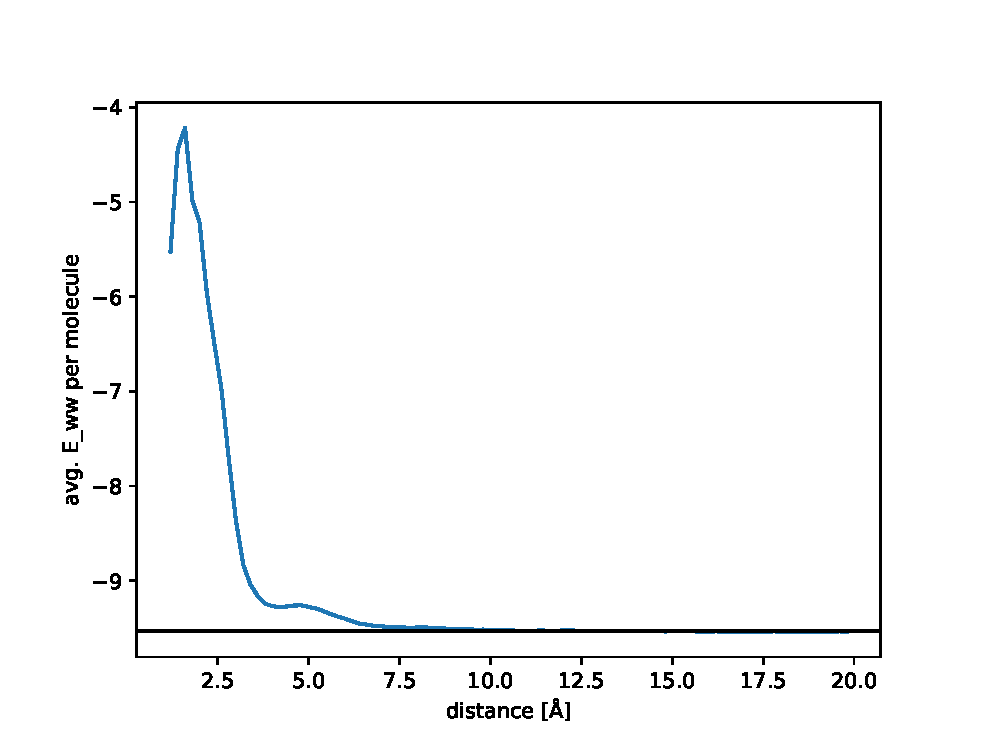
\includegraphics[width=0.8\linewidth]{figures/Eww_convergence.eps}
	\caption{Convergence of $E_{ww}$ in the complex calculation with increasing distance to the solute (streptavidin-biotin). The horizontal line shows the automatically computed reference energy.}\label{fig_ewwref}
\end{figure}

After choosing an appropriate reference value, we need to subtract this value from $E_{ww}$.
Make sure to subtract the reference from the normalized (\_norm) data.
In \software{gisttools}, this is done simply by setting \inlinecode{gist.eww\_ref}.
%In \software{gistpp}, this can be done as follows: 
%\todo{Is there some official documentation for gistpp? We should probably link that somewhere, I feel that the code presented here is not really helpful/legible without further documentation. -vah}
%\todo{This might become invalid with future GIST versions, depending on whether we adopt the COM as molecular center.} 
%\todo{Better use the population.}

%\begin{lstlisting}[style=bash]
%rho0=0.03287465
%neg_eww_ref=9.533
%gistpp -op multconst -i gist-gO.dx -opt const $rho0 \
%    -o gist-gO-abs.dx 
%gistpp -op div -i gist-Eww-dens.dx -i2 gist-gO-abs.dx \
%    -o gist-Eww-norm.dx
%gistpp -op addconst -i gist-Eww-norm.dx \
%    -opt const $neg_eww_ref -o gist-Eww-ref-norm.dx
%gistpp -op mult -i gist-Eww-ref-norm.dx \
%    -i2 gist-gO-abs.dx -o gist-Eww-ref-dens.dx
%\end{lstlisting}

Now, sum all free energy contributions to obtain the spatially resolved $\dgsolv$.
In \software{gisttools}, this is done automatically and can be accessed using the \inlinecode{A\_dens} and \inlinecode{A\_norm} data rows.

\newcommand{\coordinate}{\mathbf{r}}
\begin{equation}
	\dgsolv(\coordinate) = \Delta E_{ww}(\coordinate) + \Delta E_{sw}(\coordinate) - T\Delta S^\text{six}(\coordinate)
\end{equation}

%In \software{gistpp}, use the \inlinecode{add} command, with the same syntax as the \inlinecode{div} command used above.
After that, check whether your free energy contributions become negligible far away from the solute.
In a plot like Figure~\ref{fig_ewwref} based on the \inlinecode{A\_dens} column, the values should tend to zero.
However, it is more informative to plot the cumulative free energy contribution against the distance to the solute, to check the convergence.
It the curve flattens out, the converged value is your final $\dgsolv$\@.
Otherwise, you might need to tweak the $E_{ww}$ reference, or introduce a reference value for the entropy.

\begin{lstlisting}[style=python]
from gisttools.gist import load_gist_file
import matplotlib.pyplot as plt
# adapt eww_ref!
gist = load_gist_file("gist.dat",
    struct="solute-centered.pdb", eww_ref=-9.533)
bins, (dg, esw, eww, s) = gist.rdf(
    ["A_dens", "Esw_dens", "Eww_dens", "dTSsix_dens"],
    bins=100, rmax=20., normalize="none")
plt.plot(bins, np.cumsum(dg), label="dG")
plt.plot(bins, np.cumsum(eww), label="Eww")
plt.plot(bins, np.cumsum(esw), label="Esw")
plt.plot(bins, np.cumsum(s), label="dS")
\end{lstlisting}

The expected output of this code is shown in Figure~\ref{fig_radial_convergence}.
Especially the solvent-solvent energy is not perfectly flat, indicating that the reference value is not optimal.
%but is also complicated because the solute is charged.
Both the entropy and $E_{sw}$ can be considered converged around \SI{10}{\angstrom}.
While this is not true for $E_{ww}$, we will see below that the energy difference upon binding converges more readily than its individual contributions.
\todo{vah: Is that shown somewhere yet -> fwa?}

\begin{figure}
	\centering
	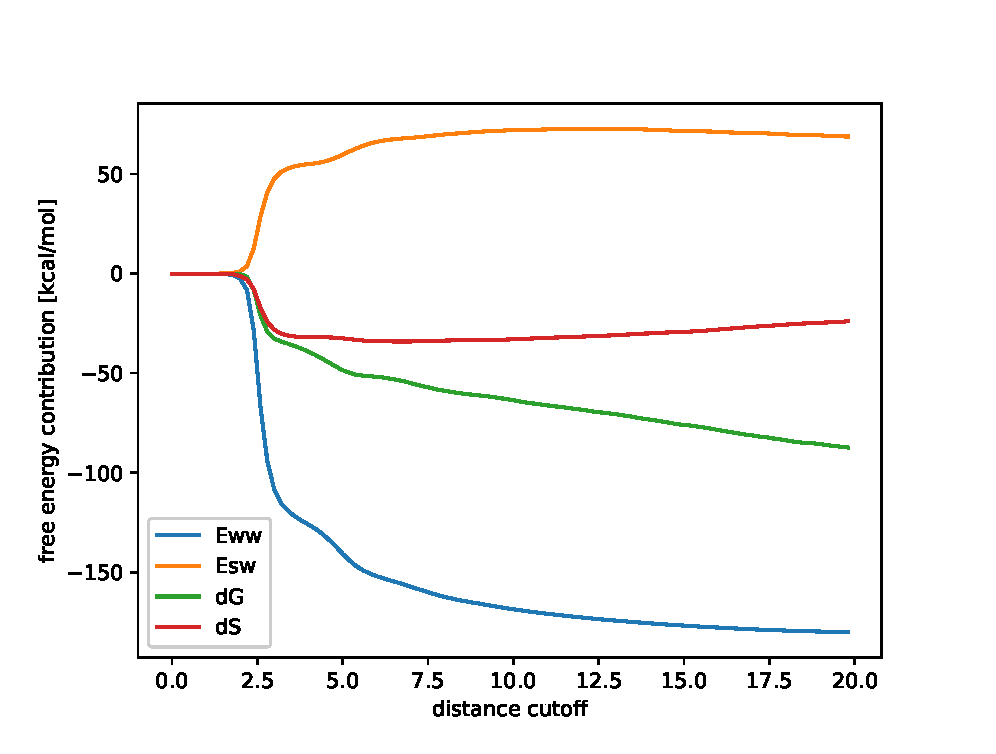
\includegraphics[width=0.8\linewidth]{figures/A_E_S_convergence.eps}
	\caption{Convergence of $\dgsolv$ and its contributions with increasing distance to the solute. All quantities cumulative, i.e., summed up to the respective radius. Computed from the biotin calculation.}\label{fig_radial_convergence}
\end{figure}

\subsubsection{Visualizing $\dgsolv$}
Next, we want to visualize the 3-dimensional contributions to the free energy of hydration, as well as the entropy and enthalpy contributions.
You can use PyMol\cite{pymol} or VMD\cite{vmd} to visualize the .dx files from GIST\@.
With \software{gistpp}, you can use the file from the convergence check. Additional OpenDX files can be produced using \inlinecode{gistpp -op makedx}.
With \software{gisttools}, you can create one using e.g., \inlinecode{gist.save\_dx("A\_dens", "A\_dens.dx")}.

It might also be interesting to visualize the average energy of a water molecule at each grid voxel.
This quantity is given by $2E_{ww} + E_{sw}$.
The energy referencing leads to non-zero normalized values where the population is zero.
While this is irrelevant for further post-processing, it is advantageous for visualization to set those empty regions to zero.
An OpenDX file can be produced using \software{gisttools} as follows:

\begin{lstlisting}[style=python]
import gisttools as gt
gist = gt.gist.load_gist_file("gist.dat",
    struct="solute-centered.pdb", eww_ref=-9.533)
gist['E_norm'] = gist['Eww_norm'] * 2 + gist['Esw_norm']
gist.loc[gist['population'] == 0, 'E_norm'] = 0
gist.save_dx('E_norm', 'gist-E-per-mol-norm.dx')
\end{lstlisting}

Visualize the free energy, the energy, and the entropy, at several isolevels.

Adapt the above PyMOL script to visualize the average energy per solvent at a positive and a negative isolevel, as well as regions of negative entropy per solvent.
The expected representation of the streptavidin binding pocket is shown in Figure~\ref{fig_binding_pocket_pymol}.

\begin{figure}
	\centering
	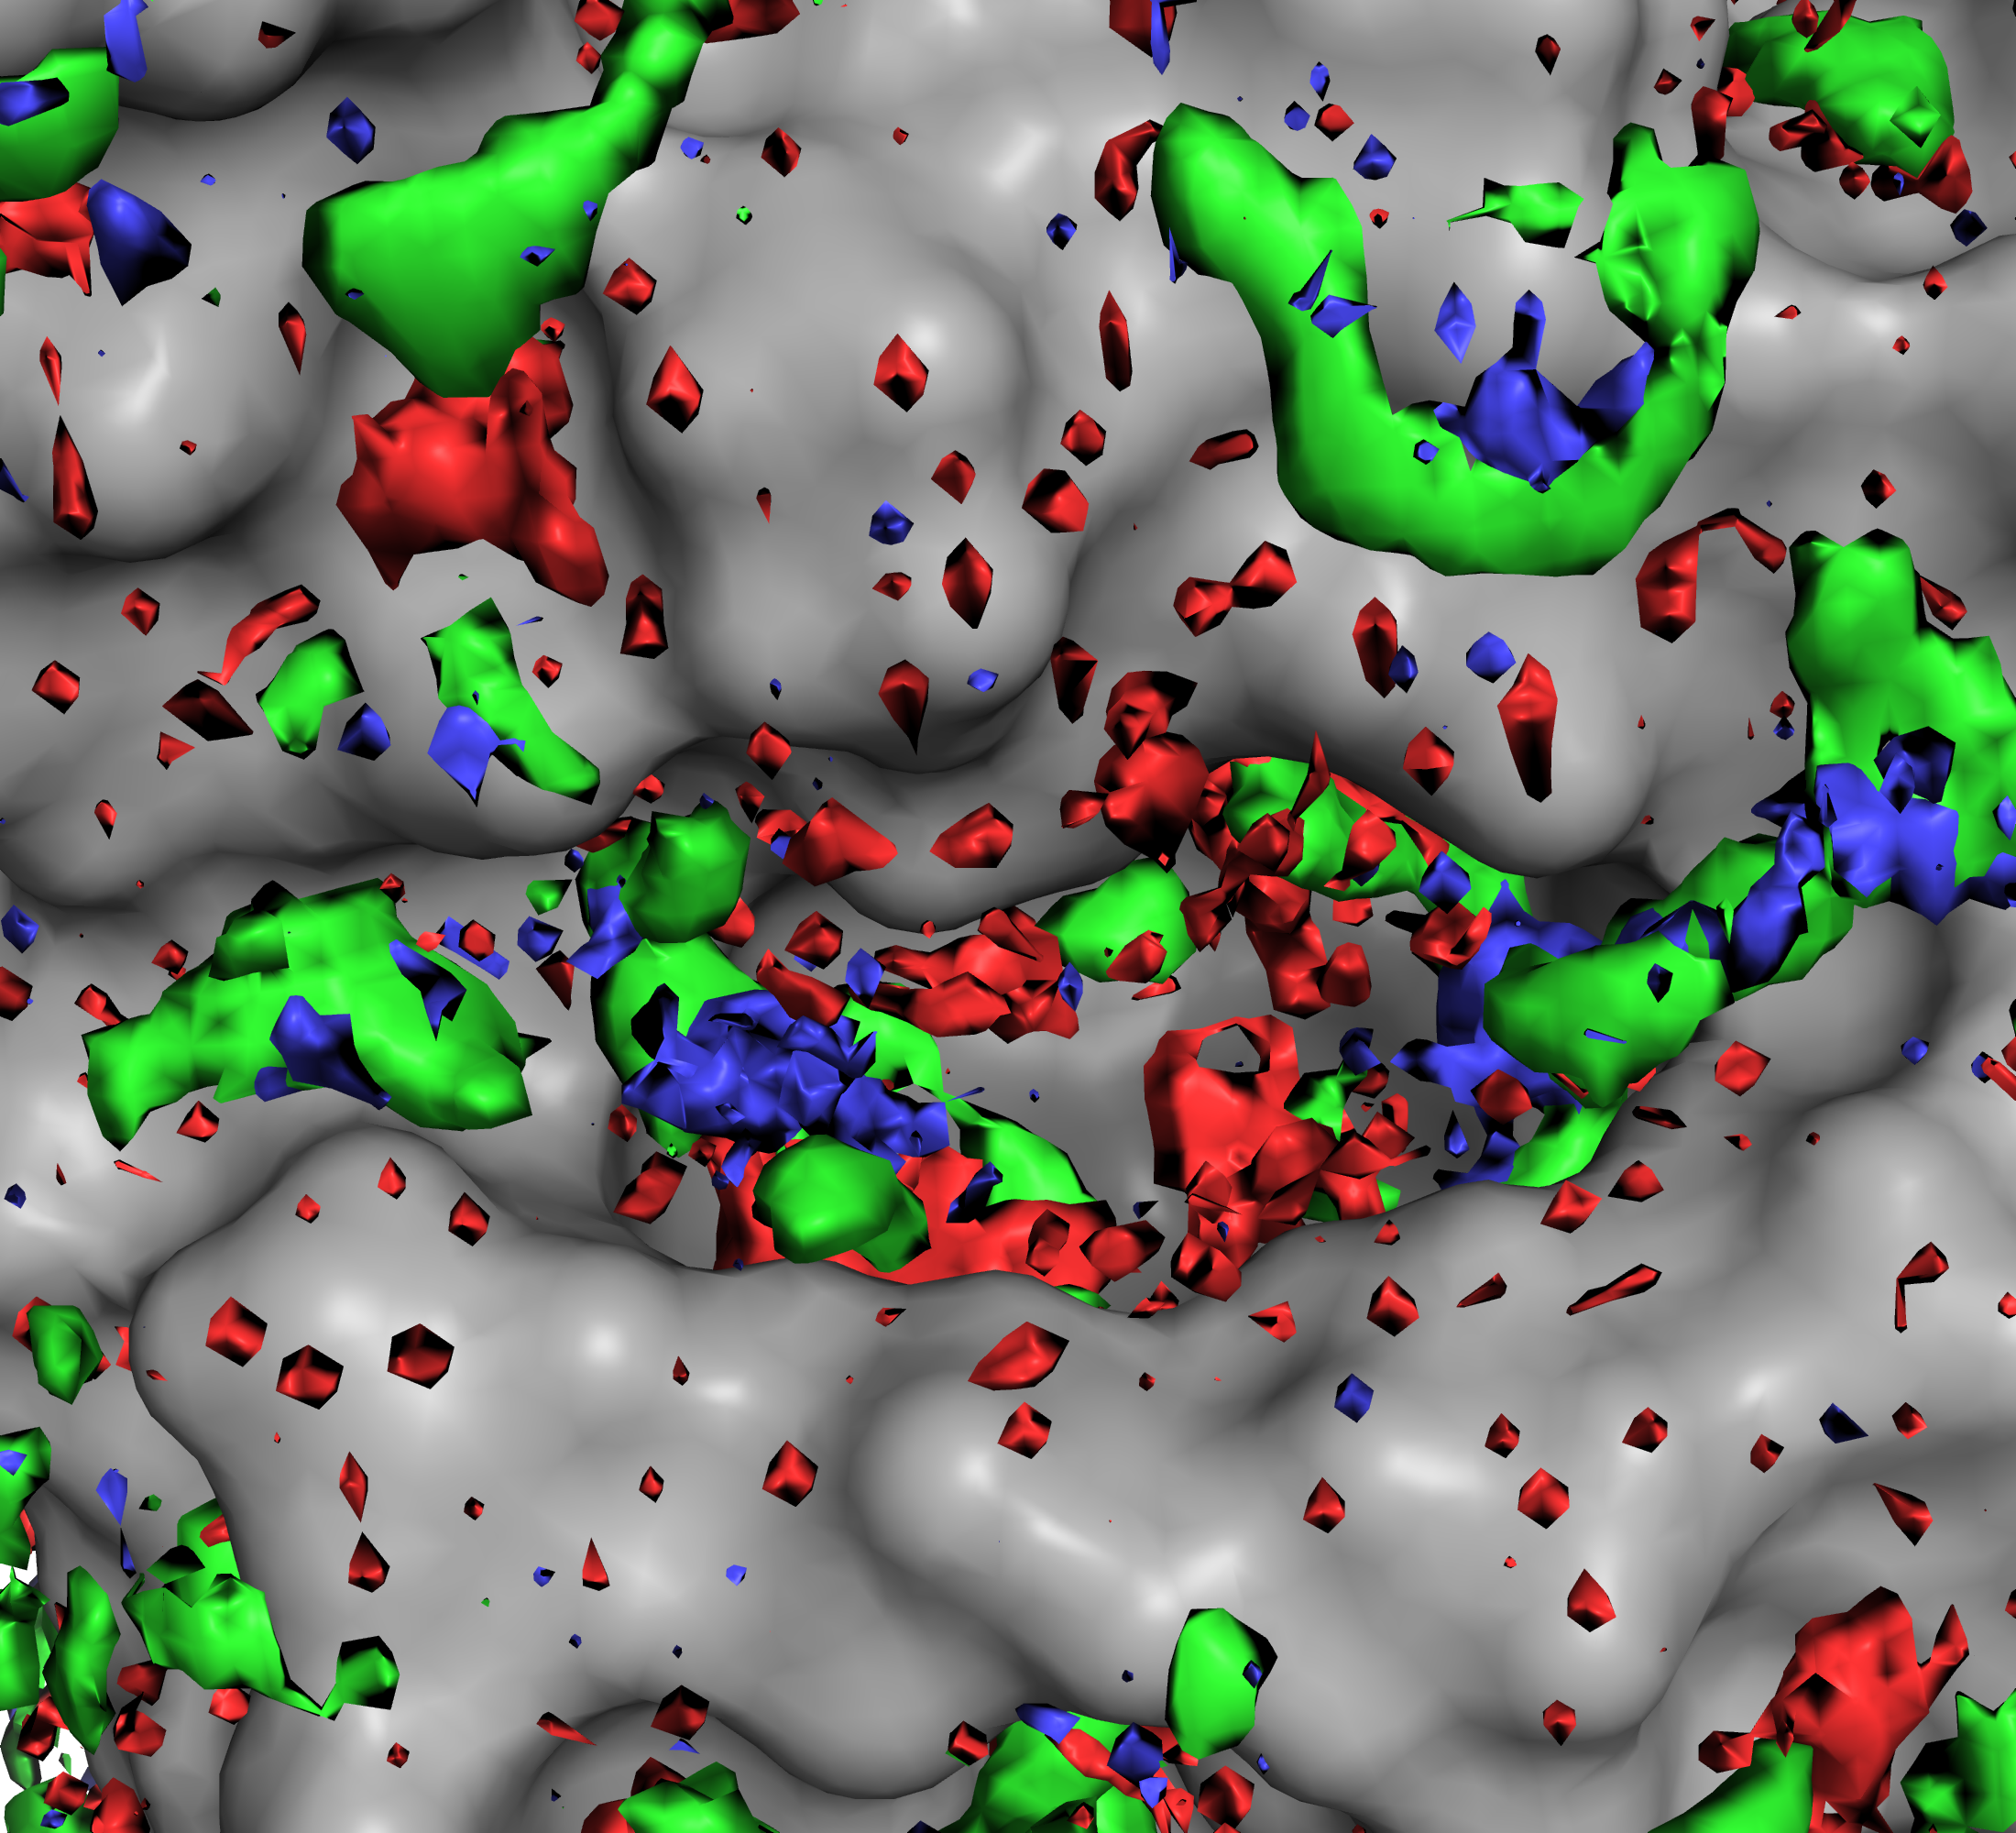
\includegraphics[width=0.8\linewidth]{figures/binding_pocket_S_-2_E_-2_E_3.png}
	\caption{Free energy contributions in the streptavidin binding pocket. Red: high solvent energy (at +3 kcal/mol). Blue: low solvent energy (at -2 kcal/mol). Green: low solvent entropy $T\Delta S^{six}$ (at -2 kcal/mol).}\label{fig_binding_pocket_pymol}
\end{figure}

You should find that there are several regions in the binding pocket that feature a high solvent energy and/or low entropy.
However, such regions also exist outside of the binding pocket, and there are also low-energy regions within the binding pocket.
Therefore, the strong affinity to biotin cannot be explained only by hydration, and the direct interaction energy also needs to be taken into account.

\subsubsection{Contribution of Hydration to Binding}
In the next step, calculate the $\dgsolv$ contributions around biotin in each system (biotin, streptavidin, and complex).
Note that our integration region does not fully reach into bulk, and some of the boundary regions are close to streptavidin. 
Therefore, our results for each system will depend on the exact position of the integration boundary. 
To avoid inconsistencies, it is important to choose exactly the same integration region for each system.
Although we kept the systems rigid, the center of mass might have been shifted during pressure equilibration.
Therefore, we align the complex structure to streptavidin and use the shifted biotin coordinates to define the integration region.

We recommend using a \software{Jupyter Notebook} for the following analyses.
The code is not explained in detail here, but should be clear after reading the previous sections.

Load the files and double check the frame numbers and reference density.
\begin{lstlisting}[style=python]
import numpy as np
from gisttools.gist import load_gist_file
import matplotlib.pyplot as plt

compl = load_gist_file('complex/gist/gist.dat', \
    struct='complex/gist/solute-centered.pdb')
print(compl.n_frames, compl.rho0)
biotin = load_gist_file('biotin/gist/gist.dat', \
    struct='biotin/gist/solute-centered.pdb')
print(biotin.n_frames, biotin.rho0)
strept = load_gist_file('streptavidin/gist/gist.dat', \
    struct='streptavidin/gist/solute-centered.pdb')
print(strept.n_frames, strept.rho0)
\end{lstlisting}
Assign reference energies and check them for plausibility.
\begin{lstlisting}[style=python]
biotin.eww_ref = biotin.detect_reference_value()
print("Biotin:", biotin.eww_ref)
strept.eww_ref = strept.detect_reference_value()
print("Streptavidin:", strept.eww_ref)
compl.eww_ref = compl.detect_reference_value()
print("Complex:", compl.eww_ref)
\end{lstlisting}

Subtract a reference entropy from the \inlinecode{dTSsix} columns.
\todo{Update with newest gisttools -> fwa}
\begin{lstlisting}[style=python]
def reference_entropy(gf):
    if 'dTSsix_unref_norm' not in gf.data.columns:
        gf['dTSsix_unref_norm'] = gf['dTSsix_norm']
        gf['dTSsix_unref_dens'] = gf['dTSsix_dens']
    gf['dTSsix_norm'] = gf['dTSsix_unref_norm'] \
        - gf.detect_reference_value('dTSsix_unref_dens')
    gf['dTSsix_dens'] = gf.norm2dens(gf['dTSsix_norm'])
reference_entropy(biotin)
reference_entropy(strept)
reference_entropy(compl)
\end{lstlisting}

Compute the atom positions that define the integration region.
For the streptavidin integral, we align the complex structure onto streptavidin and then use the biotin positions as centers.
Note that we use \software{mdtraj} here, since \software{gisttools} stores the reference structure as an \software{mdtraj} \inlinecode{Trajectory} object.
\begin{lstlisting}[style=python]
col = 'dTSsix_dens'
def select(traj, sel):
    "Slice a Trajectory by selection mask."
    return traj.atom_slice(traj.top.select(sel))
# we multiply by 10 to convert nm to Angstrom.
compl_x = select(compl.struct, biotin_mask).xyz[0] * 10.
biotin_x = select(biotin.struct, biotin_mask).xyz[0]*10.
aligned = compl.struct[:].superpose(strept.struct, \
    atom_indices=strept.struct.top.select(strept_mask))
aligned = select(aligned, biotin_mask)
strept_x = aligned.xyz[0] * 10.

bins, biotin_rdf = biotin.rdf( \
    col, centers=biotin_x, bins=100, rmax=24)
bins, strept_rdf = strept.rdf( \
    col, centers=strept_x, bins=100, rmax=24)
bins, compl_rdf = compl.rdf( \
    col, centers=compl_x, bins=100, rmax=24)
\end{lstlisting}

Now, subtract the monomer rdfs from the complex, and compute the integrals.
If you also visualize the individual rdfs, you will notice that the difference converges much better with increasing radius than the contributions.
This is because the cutoff contains regions that are close to the atom, since the integration region does not comprise the whole protein.

\begin{lstlisting}[style=python]
difference = compl_rdf - biotin_rdf - strept_rdf
cutoff = 12
integral = difference[bins < cutoff].sum()
print("Integral = {}".format(integral))
plt.plot(bins, np.cumsum(difference))
plt.axvline(cutoff)
plt.xlabel('distance to biotin [Å]')
plt.ylabel('dG contribution [kcal/mol]')
\end{lstlisting}
% \todo{\$\textbackslash AA\$ should produce an angstrom sign in matplotlib (what a pain to have this printed out in \LaTeX\ tho) -vah} -- Å produces an angstrom sign ;-)
Compute the energy (\inlinecode{Eall}) and entropy (\inlinecode{dTSsix}) contributions separately.
You will find that the energy disfavors binding, because we do not yet include the interaction energy between biotin and streptavidin.

You can also plot the difference between the complex and monomer contributions against the distance to biotin, using the complex coordinates for the holo structure.
The expected result is shown in Figure~\ref{fig-dg-sums}.

\begin{figure}
	\centering
	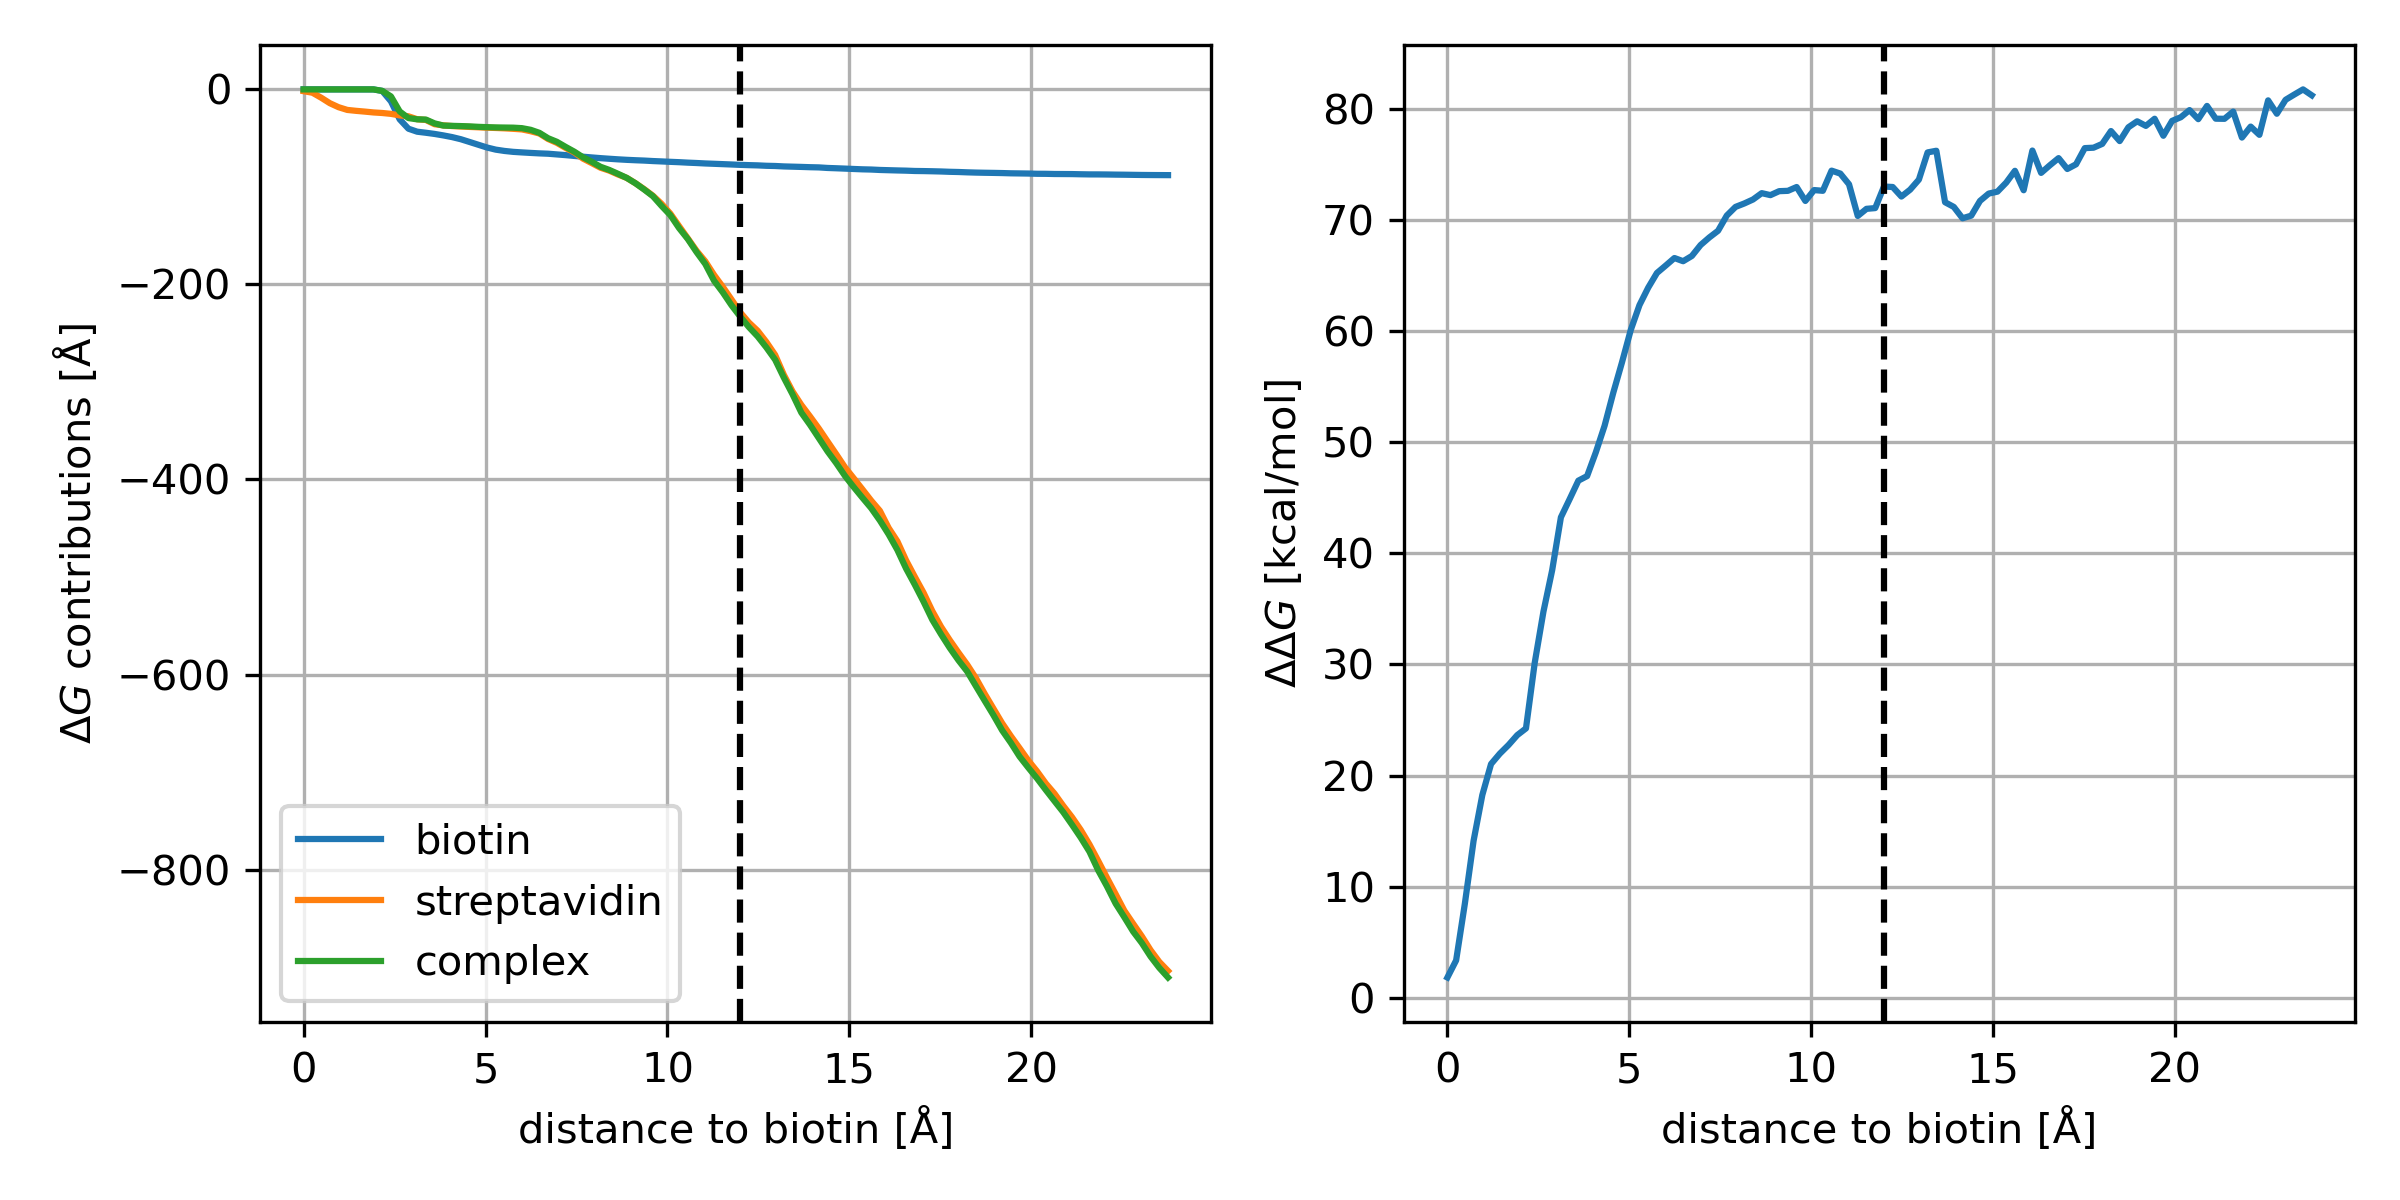
\includegraphics[width=1.0\linewidth]{figures/deltaG-difference.png}
	\caption{TODO caption}\label{fig-dg-sums}
\end{figure}

Using the \inlinecode{energy} command in \software{cpptraj}, you can compute this interaction energy.
We recommend using PME in combination with PME-GIST, but not with GPU-GIST\@.
An example \software{cpptraj} input might look like:
\begin{lstlisting}[style=cpptraj]
parm solvated.parm7
trajin md-01.nc 1 last 100
energy complex ^1,2 # etype pme
energy strept ^1 # etype pme
energy biotin ^2 # etype pme
go
diff = complex[total] - strept[total] - biotin[total]
writedata energy.dat diff complex[total] \
strept[total] biotin[total]
avg(complex[total])
avg(strept[total])
avg(biotin[total])
avg(diff)
\end{lstlisting}

It has been shown \cite{Chen2021,Waibl2022-gist-solvents} that the solvation entropy in water is best approximated by 0.6 times the first order entropy.
Also compute the scaled entropy and check the effect on the binding affinity.
The expected results are summarized in Table~\ref{tab_dg_monomers_dimer}.
%\todo{Table 1 is placed quite akwardly at the moment for me, maybe enforce its position? -vah. Ok? -fwa}

\begin{table}[h]
	\caption{Free energy contributions for the monomers and the dimer in kcal$\cdot$mol$^{-1}$. ``Diff'' is calculated as $E^\text{internal} + \Delta E^\text{GIST} - \Delta S^\text{scaled}$.}\label{tab_dg_monomers_dimer}
	\small
	\begin{tabular}{@{}lrrrrr@{}}
		\toprule
		System       & E(internal) & $\Delta E^\textit{GIST}$ & $T\Delta S^\textit{GIST}$ & $T\Delta S^\textit{scaled}$ & Diff \\
		\midrule
		complex      & -1303.4 & -361.2 & -233.1 & -139.9 & -1524.7 \\
		streptavidin & -1180.7 & -360.8 & -242.4 & -145.4 & -1396.1 \\
		biotin       & -24.0   &  -98.1 &  -35.1 &  -21.1 &  -101.0 \\
		Diff         & -98.7   &   97.7 &   44.4 &   26.6 &   -27.6 \\
		\bottomrule
	\end{tabular}
\end{table}

Even though streptavidin-biotin is known to be a very stable complex, the solvation energy favors the dissociation.
This is expected: if the molecules were not able to form any interactions, but interacted fully with the water, they would not form a complex.

In this case, we find that the energy of solvation and the internal energy of the complex more or less cancel out, indicating that binding is largely entropy-driven in this case.
At first, this is surprising, since isothermal titration calorimetry (ITC) of biotin-streptavidin shows strong enthalpic binding contributions \cite{mpye2020-biotin-itc,hyre2006-biotin-itc}.
However, we do not take the conformational transition of the streptavidin binding pocket into account.

Prior computational studies suggest a $\Delta G$ of \SI{-26.6}{\kilo\calorie\per\mole} for the binding of biotin into the closed conformation of streptavidin \cite{Bansal2018-biotin}.
This indicates that our result is in good agreement with literature.
To improve the agreement with ITC measurements, the conformational changes of the binding pocket should be included.

\subsubsection{Further steps}
In this tutorial, we obtained a value for the binding of biotin into the closed conformation of the streptavidin binding pocket.
To investigate the effect of different conformations on the binding affinity, you can perform molecular dynamics simulations of the complex and/or monomers and perform GIST on multiple cluster representatives.
To include the effect of lid closing in the binding process, free energy calculation methods such as umbrella sampling can be used.

To speed up the calculation, smaller GIST grids could be used by focusing on the binding pocket, or by rotating the molecule by its principal axes to fit the cuboid grid more exactly.
However, this should be done \emph{before} the MD, since rotating the trajectory damages the periodic box information \todo{@Dan: is this still the case?}.

\section{Recent developments}
In recent years, several updates to the original GIST implementation have been published.
The basic functionality of the program, however, has not been changed.
In this chapter, we will shortly present each of those updates.
\subsection{GPU implementation}
In Reference~\cite{Kraml2020}, a GPU implementation of the energy calculation was presented, which typically increases the speed by 1--2 orders of magnitude.

If \software{cpptraj} is compiled with GPU support, the energy calculation uses the GPU automatically, without any additional input.
However, PME-GIST is not supported on the GPU, and no GPU code will be used when specifying \inlinecode{pme}.

\subsection{PME implementation}
In Reference~\cite{Chen2021}, a PME implementation of the GIST energy was presented.
For typical systems, this implementation is slightly slower than GPU-GIST, but much faster than the original CPU code.
Furthermore, PME-GIST offers the best agreement between GIST energies and those observed in an MD simulation.

To run PME-GIST, the \inlinecode{pme} flag to \inlinecode{gist} can be used in \software{cpptraj}.
The output will contain two additional columns: \inlinecode{PME\_dens} and \inlinecode{PME\_norm}.
They contain the potential of solute and solvent evaluated at the solvent positions and divided by two.
Furthermore, the \inlinecode{Eww} and \inlinecode{Esw} columns are also computed using PME, and are reported as usual.
For typical use cases, we recommend using \inlinecode{Eww} and \inlinecode{Esw} over the \inlinecode{PME} column.

\subsection{GIST with non-water solvents}
In References~\cite{Kraml2020,Kamenik2020-gist-macrocycles,Waibl2022-gist-solvents}, an extension of GIST towards solvents other than water is described.

To run a GIST calculation in a solvent other than water, use \inlinecode{solute} with a \software{cpptraj} selection mask.
All other molecules will be treated as solvent.
If there are multiple solvent species, also use the \inlinecode{solventmols} flag as described in Section~\ref{sec-salt-water}.

The code will automatically choose three atoms per molecule to define the solvent orientation, and print this selection to the output.
Sometimes, however, the automatic selection is not optimal.
For instance, in methanol one can either incorporate the C--H bonds or the O--H bond in the selection.
The latter is probably more relevant since it can incorporate hydrogen bonding effects.
Assuming that the alcohol hydrogen is called H1, this could be specified as follows:

\begin{lstlisting}[style=cpptraj]
gist gridcntr <x> <y> <z> \
griddim <Nx> <Ny> <Nz> gridspacn <val> \
solute ^1 rigidatoms O1 H1 C1
\end{lstlisting}

Note that the central atom of the \inlinecode{rigidatoms} selection goes first.

\subsection{GIST with salt-water mixtures}
\label{sec-salt-water}
In \cite{Waibl2021-gist-salt}, an extension of GIST was presented that can use salt-water mixtures as a solvent.
This allows treating salting-out effects, although it was shown that the salting-out coefficient is over-predicted by GIST because of the first-order entropy approximation.
Generally, GIST should be able to treat arbitrary solvent mixtures as long as each molecule is sufficiently rigid.

In the \software{cpptraj} implementation of GIST, the \inlinecode{solute} keyword specifies which components of the system are treated as a solute.
Everything else will be treated as solvent.
If the solvent contains more than one molecular species, a list of solvent molecule names (i.e., ``\inlinecode{solventmols WAT,NA,CL}'') must be specified.
For each molecule in this list, densities (e.g., \inlinecode{g\_mol\_NA}) and energies (e.g., \inlinecode{Eww\_mol\_NA}) will be computed and written to .dx files.
Note that, e.g., \inlinecode{Esw\_mol\_NA} contains the interactions of every ``\inlinecode{NA}'' molecule with the solute, and \inlinecode{Esw\_mol\_NA} contains the interactions among ``\inlinecode{NA}'' molecules as well as their interactions with all other solvents, divided by 2 to account for double counting.
Furthermore, the first molecule in this list will be treated as the main solvent, for which first-order entropy values will be computed.

For instance, a GIST calculation in salt water, including the first-order water entropy, can be run as follows:

\begin{lstlisting}[style=cpptraj]
gist gridcntr <x> <y> <z> \
griddim <Nx> <Ny> <Nz> gridspacn <val> \
solute !(:WAT,NA,CL) solventmols WAT,NA,CL
\end{lstlisting}

The current implementation of the entropy calculation in \software{cpptraj} requires at least 3 atoms in the main solvent.
To compute the first-order entropy of the ions, as well as an approximate second order entropy, Python code is available on \url{https://github.com/liedllab/second-disorder}.

\section{Visualization}

\subsection{Visualizing DX files}
A minimal PyMOL input to visualize a dx file is shown here.
For reference, an input structure is loaded from a file named \inlinecode{streptavidin.pdb}.
The oxygen density is visualized at an isolevel of 2 (i.e., twice the reference density).
The expected output is shown in Figure~\ref{fig-streptavidin_gO}.

% The current font makes the O look like a tofu / placeholder
\begin{lstlisting}[style=pymol]
load streptavidin.pdb
as surface
color gray70, streptavidin
load gist-gO.dx, gO
isomesh gO_high, gO, 2
color slate, gO_high
\end{lstlisting}


\begin{figure}
	\centering
	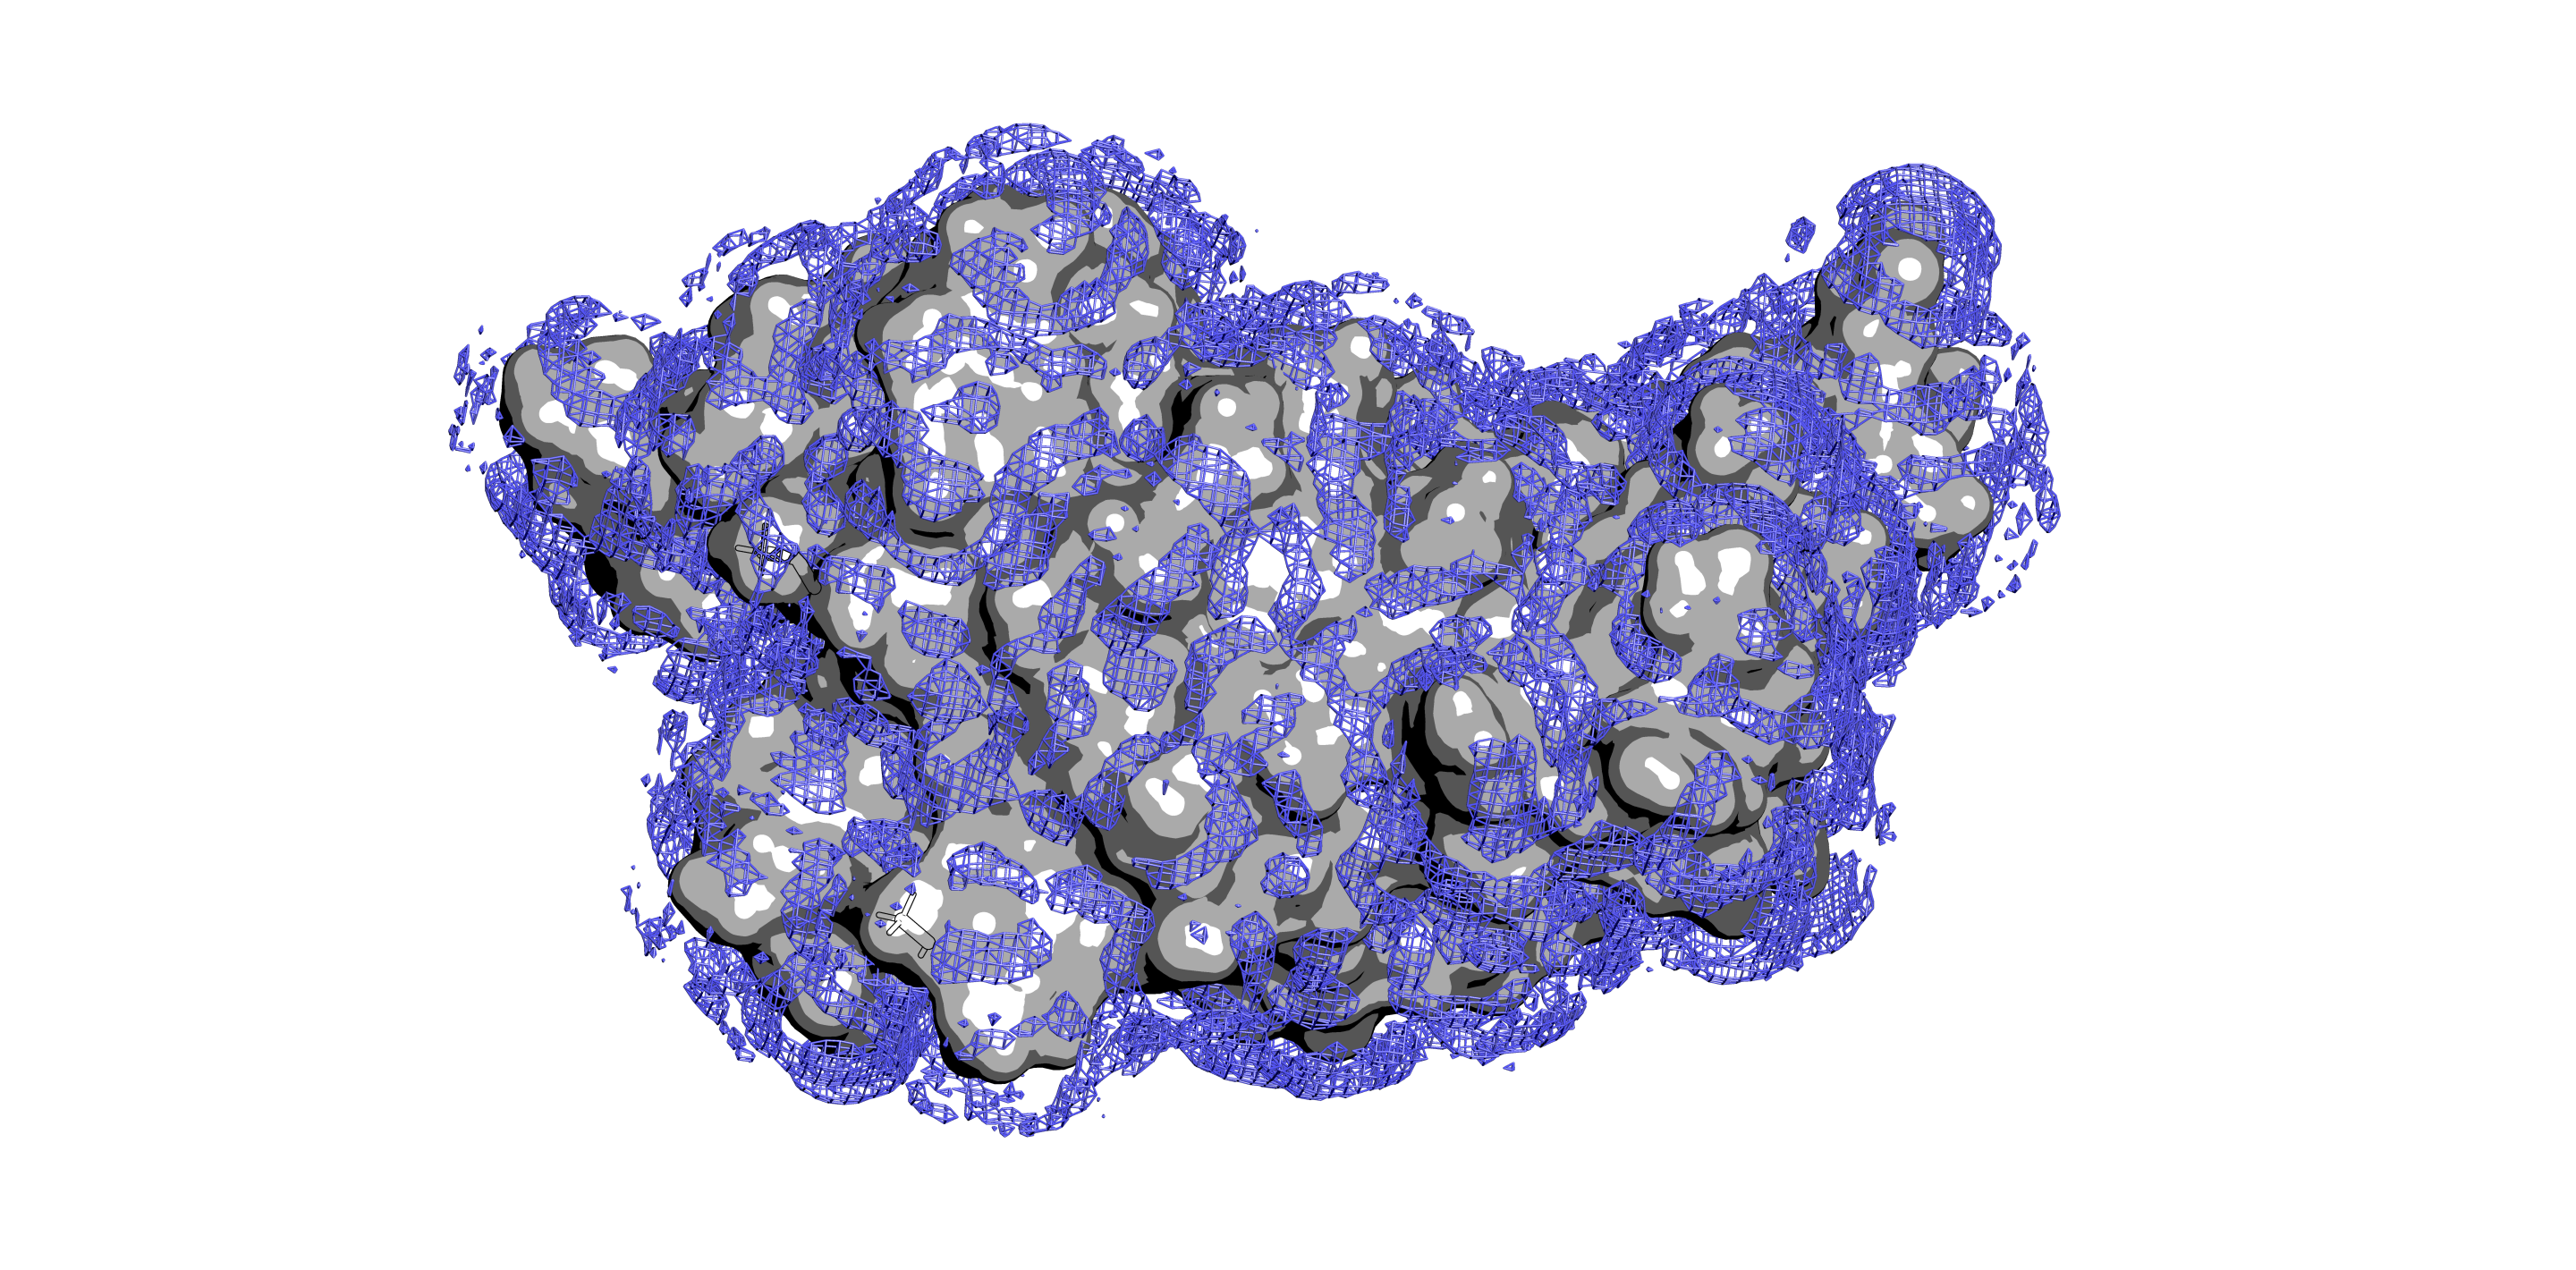
\includegraphics[width=1.0\linewidth]{figures/streptavidin_gO_high_surf.png}
	\caption{Oxygen density around streptavidin at an isolevel of twice the reference density}\label{fig-streptavidin_gO}
\end{figure}

\subsection{Solvent Accessible Surface Area (SASA)}

The solvent accessible surface (SASA) represents the interface between regions that are occupied by the solute, and those which can be accessed by the solvent.
GIST provides a very natural way of creating a SASA using an isosurface of the oxygen density gO.
It can be visualized in PyMOL.
The expected output is shown in Figure~\ref{fig-streptavidin_sasa}.

\begin{lstlisting}[style=pymol]
load ../gist.pdb
load ../gist-gO.dx
isomesh sas, gist-gO, 0.1
\end{lstlisting}

\begin{figure}
	\centering
	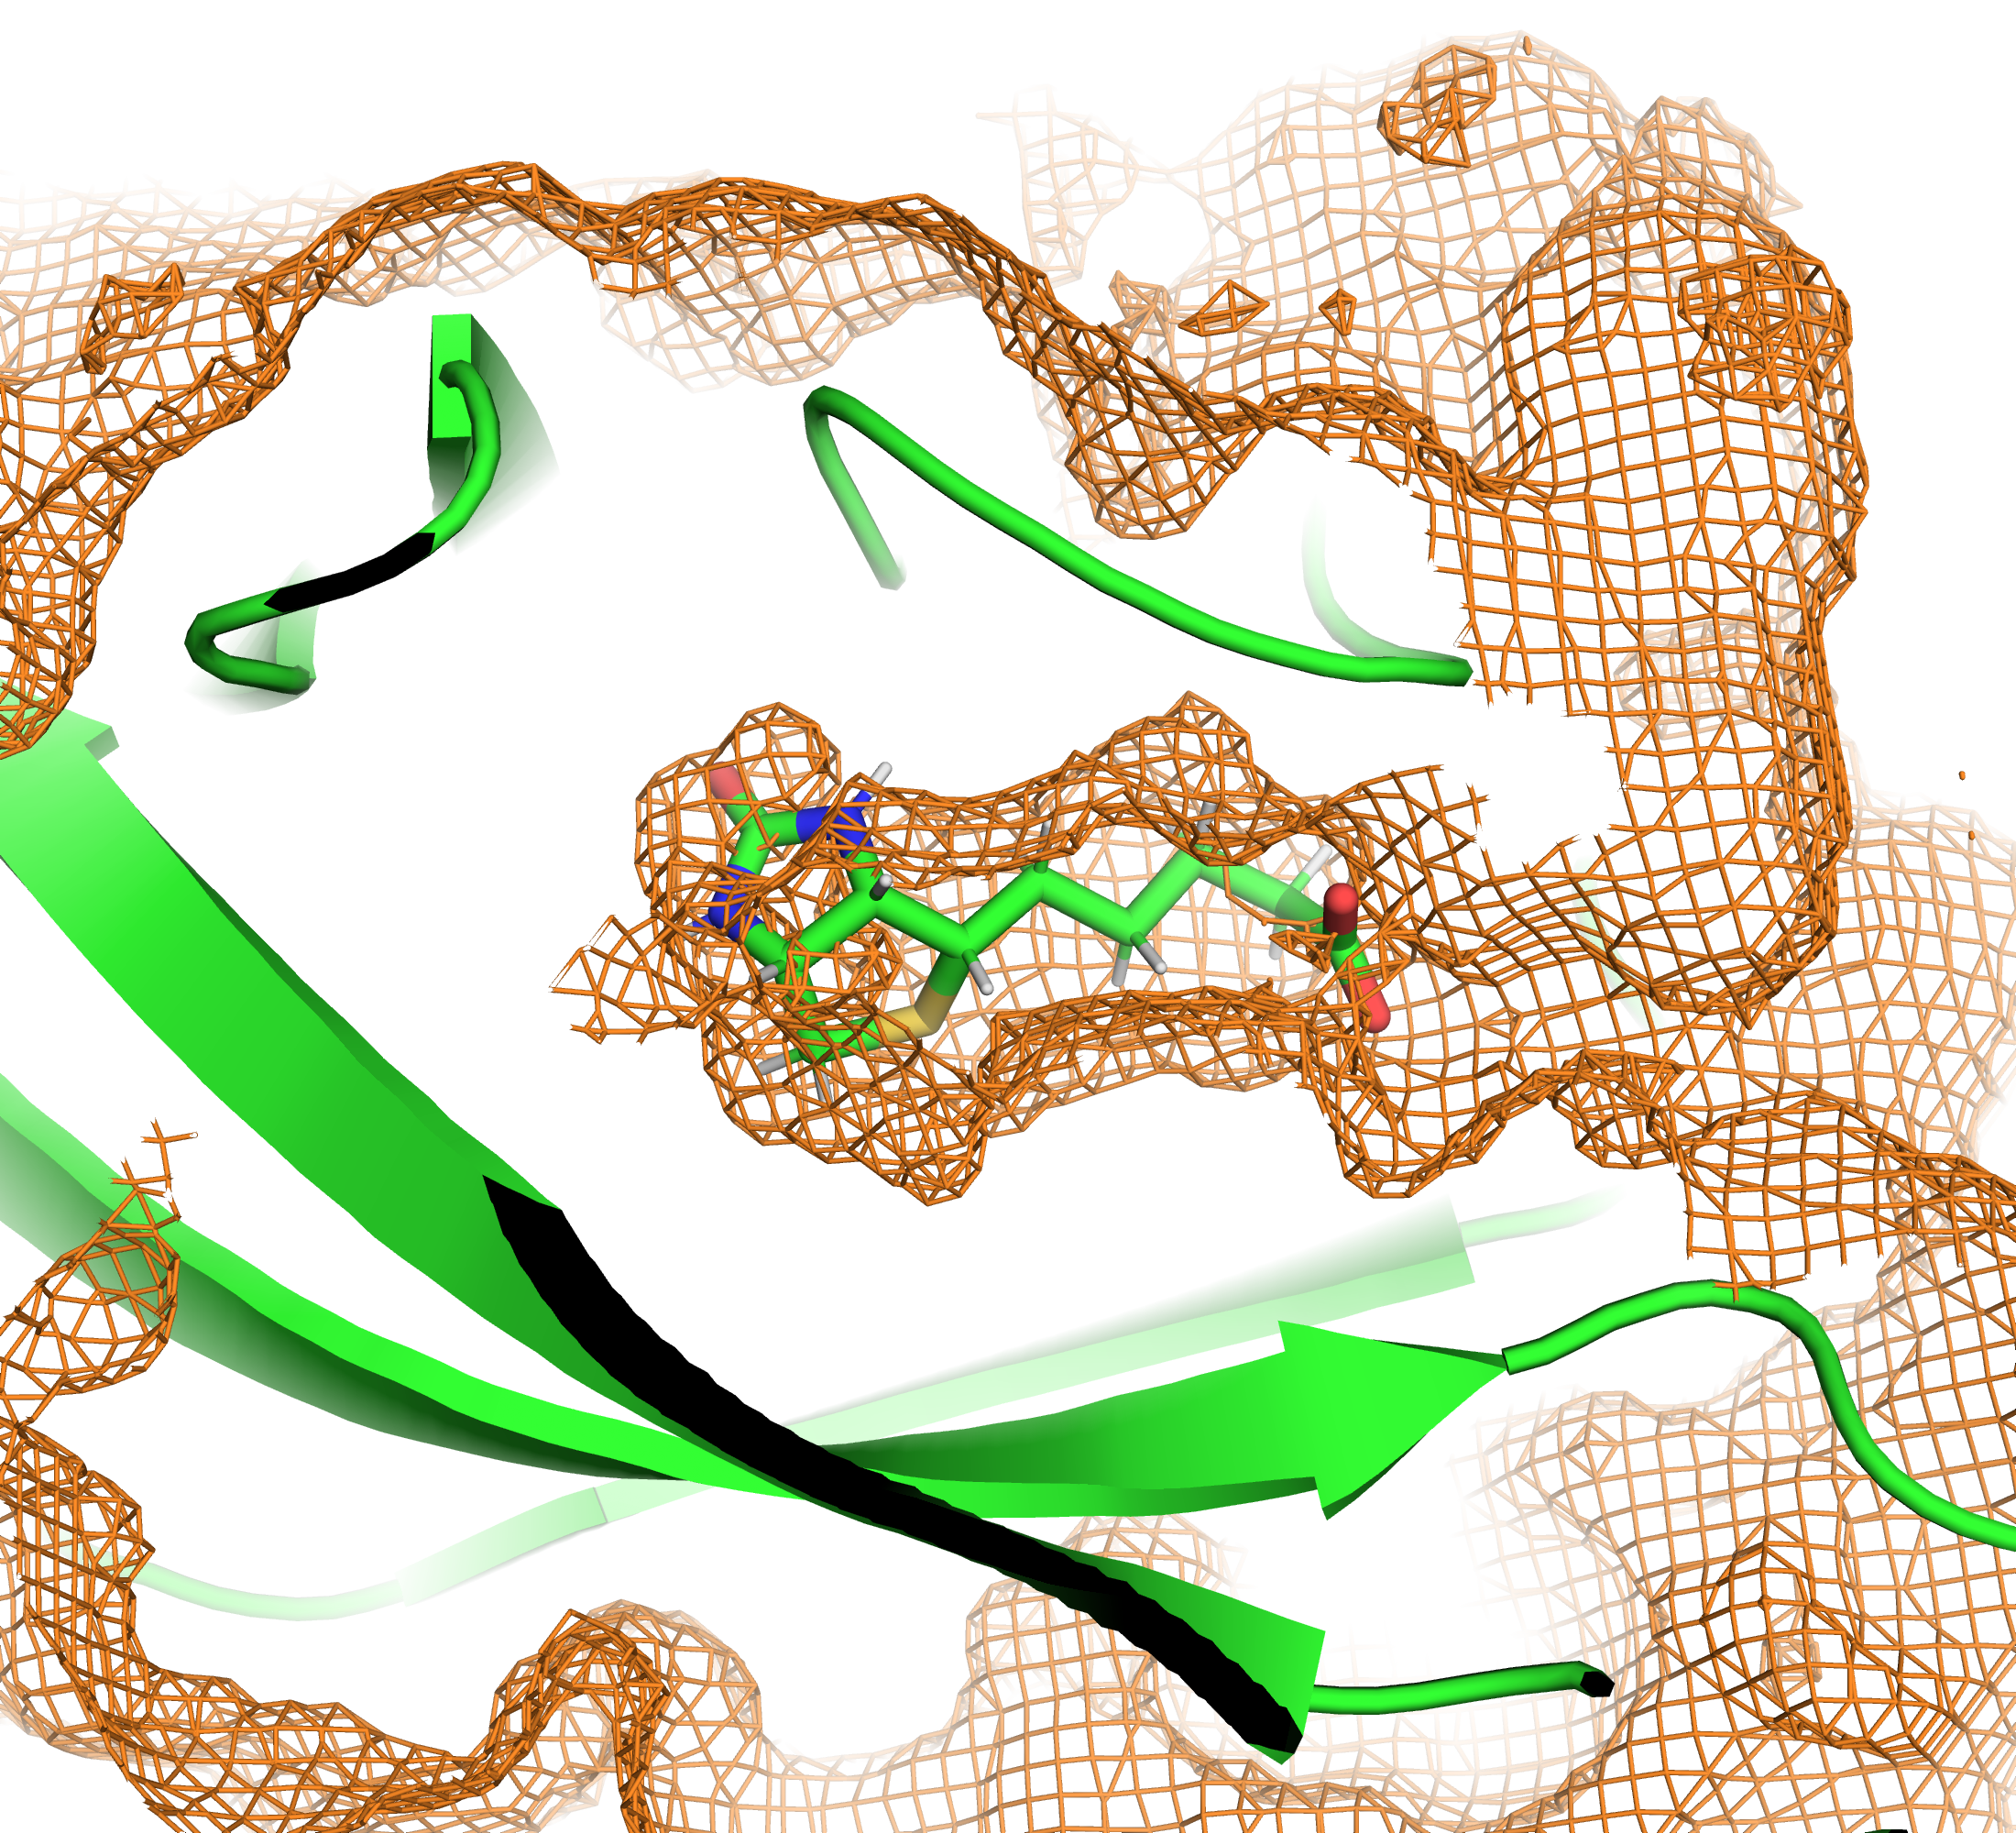
\includegraphics[width=1.0\linewidth]{figures/sasa-simple.png}
	\caption{SASA for streptavidin focused on the binding pocket}\label{fig-streptavidin_sasa}
\end{figure}

Here, the SASA was generated from a simulation of the holo protein structure.
When the ligand is placed in the binding pocked, all atoms are within the SASA. 

\subsection{Defining the binding pocket}
Specific regions in a protein can be defined to calculate the thermodynamic quantities for that region.
This is significant specially when calculating the properties of water that will be expelled when a ligand binds to the protein.

For example, voxels that are part of the binding pocket can be defined using a ligand molecule and a distance criteria. In \software{gistpp}, voxels that are within the distance criteria from any ligand heavy atom is considered as part of the region. The resulting file is a binary file and can be visualized using \software{pymol}. \todo{Not GISTPP}

\begin{lstlisting}[style=bash]
gistpp -op defbp -i gO.dx -i2 ligand.pdb 

-opt const 3.5 -o gO_3.5.dx
\end{lstlisting}

Here, the binding pocket includes all voxels within \SI{3.5}{\angstrom} of the heavy atoms of biotin. 

\begin{figure}
	\centering
	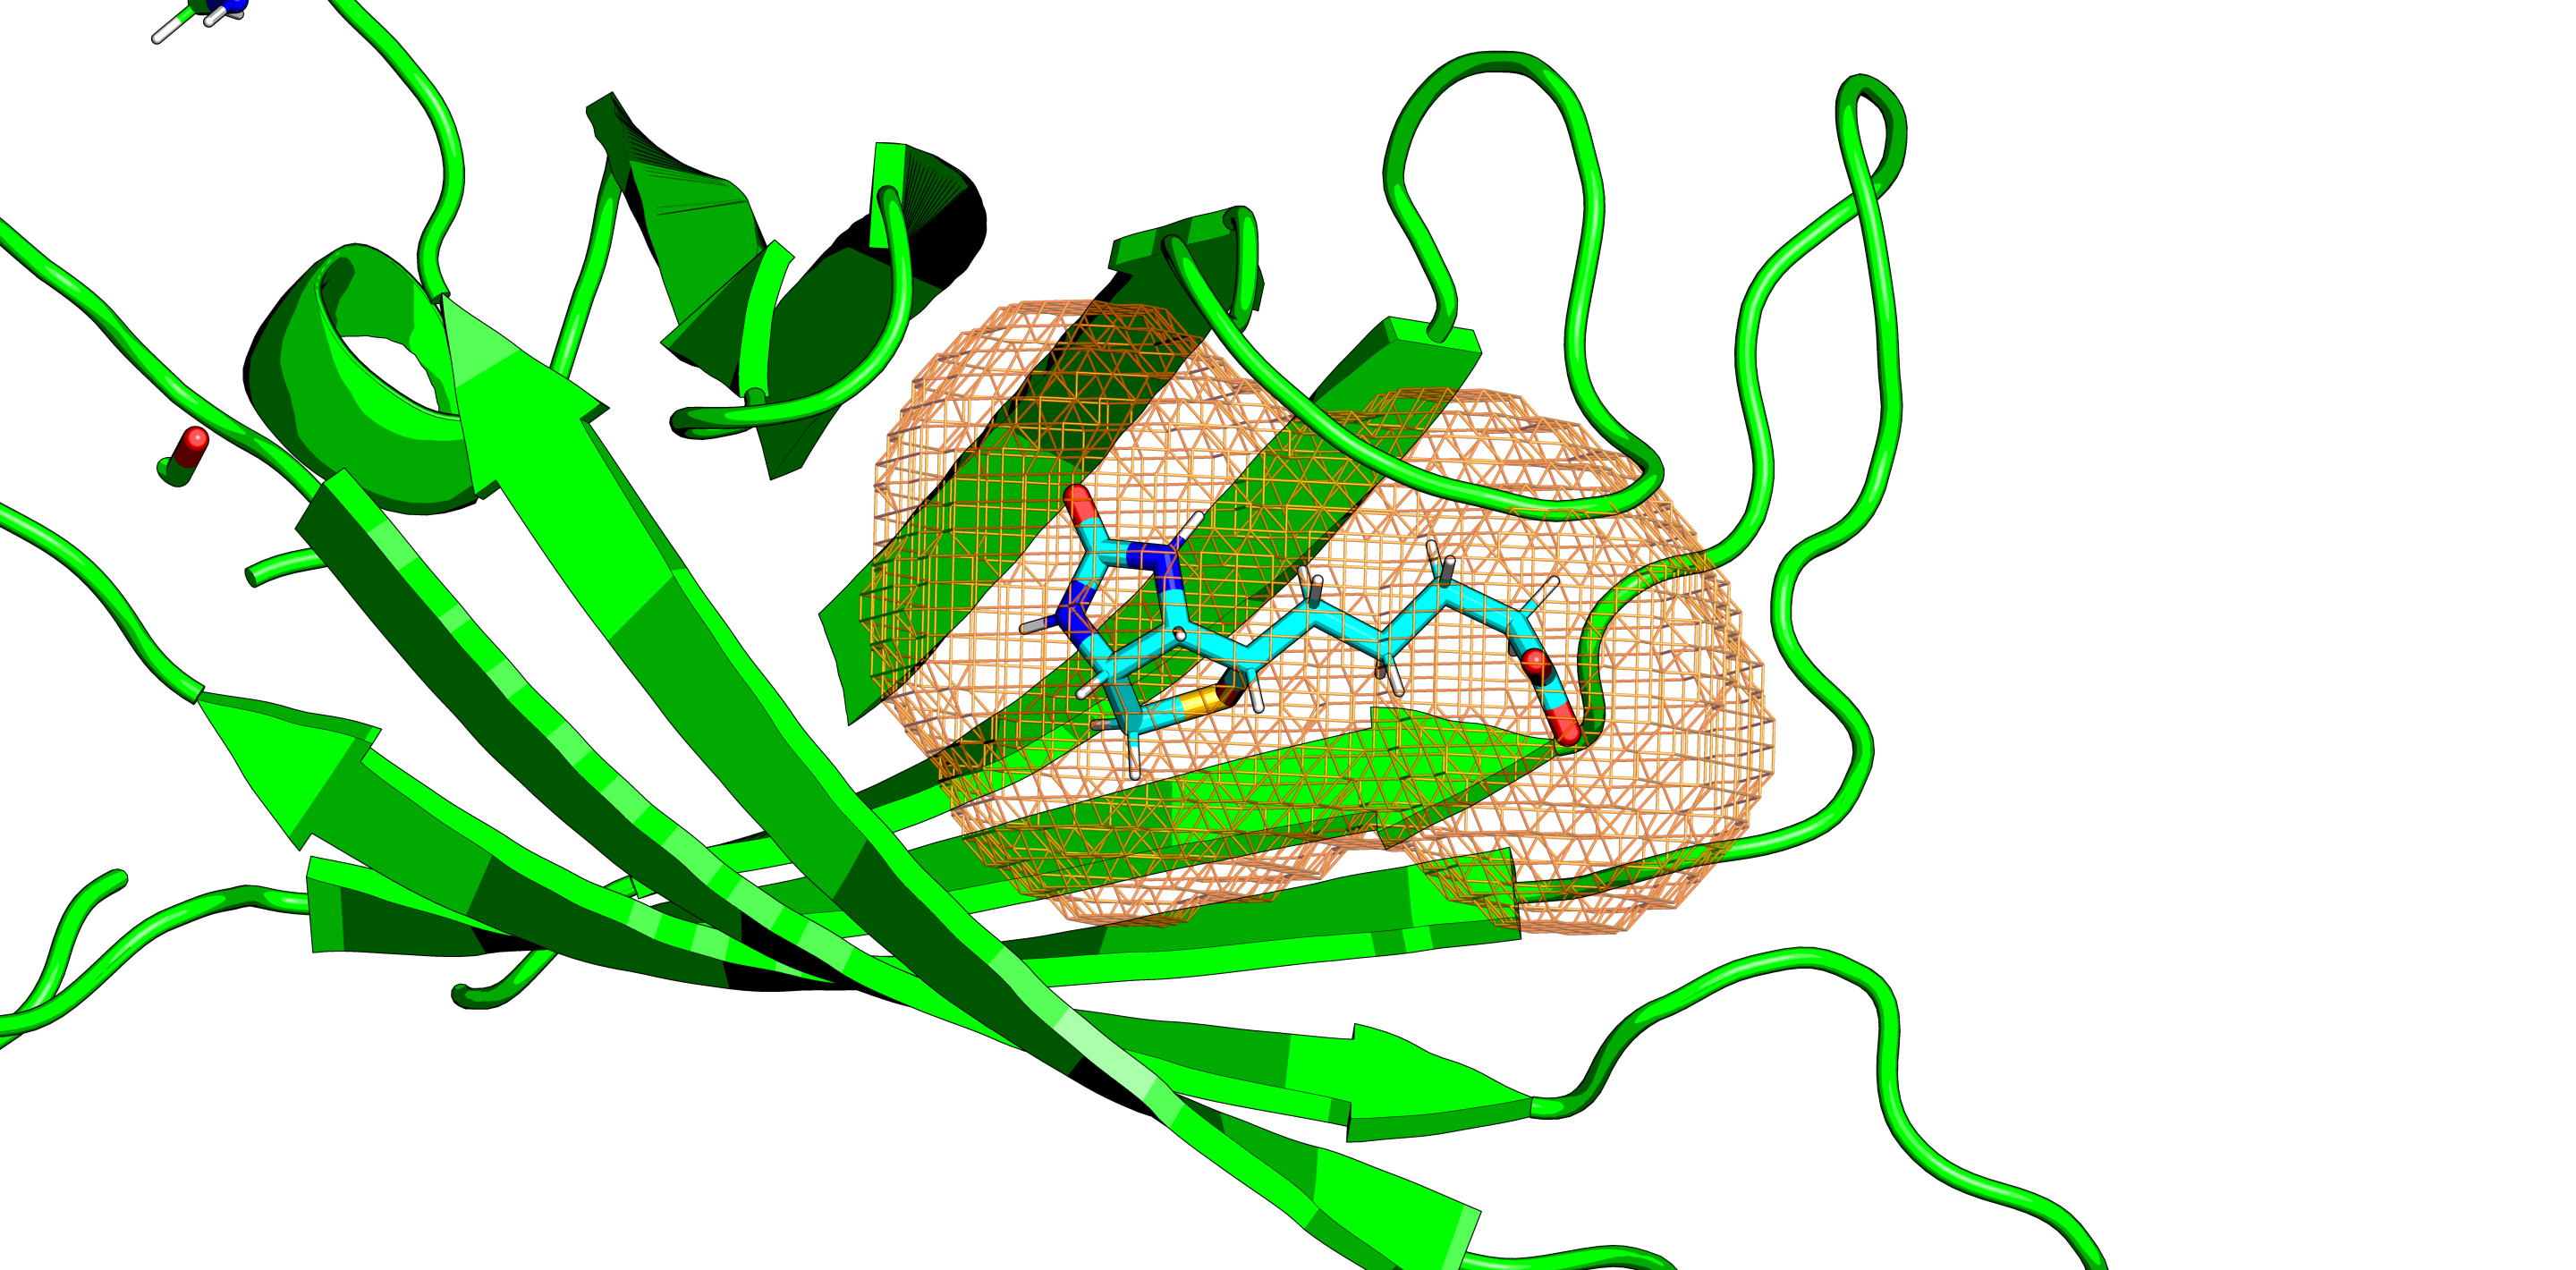
\includegraphics[width=1.0\linewidth]{streptavidin_bp_close.png}
	\caption{Volume of streptavidin defined around \SI{3.5}{\angstrom} of biotin. }\label{streptavidin_volume}
\end{figure}

\section{Theory}
\label{sec:theory}
GIST is an implementation of inhomogeneous fluid solvation theory (IST) \cite{Lazaridis1998} that discretizes the free energy of solvation $\dgsolv$ on a three-dimensional grid. 
It was first devised by Nguyen et al.\ \cite{Nguyen2012} and its implementation in \software{cpptraj} was thoroughly described by Ramsey et al.\ \cite{Ramsey2016}.
Here, we only provide a short overview of the theory behind GIST.
For more detailed information, we recommend one of the more recent publications on developments in GIST \cite{Kraml2020,Chen2021}.

\subsection{Solvation Entropy}

%\begin{equation}
%	\Delta S_\textit{solv} = \Delta S_\textit{sw} + \Delta S_\textit{ww}
%\end{equation}
%Here the solvation entropy is approximated from the contribution of solute-water interaction. 
%\textbf{STILLNEEDS REVISON + ADD CITATIONS} The quantity $k_\textit{b}$represents the Boltzman constant, 
%$\rho^\textit{o}$ is the bulk number density, $g_\textit{sw}\left(\textbf{r},\omega \right)$ is the solute-water 
%pair correlation function in the solute's frame of reference, \textbf{r} is the coordinates of the oxygen atom of the water molecule,  
%$\omega$ represents the Euler angles, and $\frac{1}{8\pi^2}$ is the volume of the orientational space, which acts as a normalization constant.
%In bulk and in regions where the orientational 
%entropy is uniform, the quantity $g_\textit{sw}\left(\textbf{r},\omega \right)$ is unity which leads to the first-order solvation entropy of 
%bulk to be zero. Also, this quantity reaches unity as the distance from the solute molecule increases which leads for the calculation of 
%the solvation entropy to be an approximation of the integral around the solute atom. 

IST expresses the free energy of solvation in terms of the solvent density in a coordinate system defined by the solute.
The solute is kept fixed in space, following the standard solvation process established by Ben-Naim \cite{ben-naim-book}.

For the entropy, this leads to an infinite expansion of correlations of increasing order.
In a slightly simplified view, the first order is the solvent density $g_\textit{sw}\left(\textbf{r},\omega \right)$ at each position $\textbf{r}$ and orientation $\omega$.
The first-order entropy omits all solvent-solvent (and higher) correlations, while the solute-solvent correlation is taken into account because the coordinates are relative to the solute.
Thus, it is called the solute-water entropy $S_{sw}$.
%The second order is the pair density, i.e., the probability of finding two solvent molecules in positions $\textbf{r}$ and $\textbf{r}^\prime$.

The solvent density is expressed relative to the bulk density $\rho^0$. %$g_\textit{sw}\left(\textbf{r},\omega \right)$ is the solute-water 
%pair correlation function in the solute's frame of reference, \textbf{r} is the coordinates of the oxygen atom of the water molecule,  
%$\omega$ represents the Euler angles, and 
The entropy integral is also normalized by $8\pi^2$, which is the volume of the orientational space.
In bulk or at a high distance to the solute, the quantity $g_\textit{sw}\left(\textbf{r},\omega \right)$ approaches one, which leads to zero first-order entropy. 
Therefore, no reference entropy is needed unless there is a numeric bias, e.g., when the MD frames are statistically dependent because the time between them is insufficient.
\begin{equation}
	\Delta S_\text{solv}
	\approx \Delta S_\textit{sw}
	\newcommand{\gro}{g_{sw}(\textbf{r},\omega)}
	\equiv -R \frac{\rho^0}{8\pi^\textit{2}} \int \gro \ln\gro d\textbf{r}d\omega
\end{equation}

\subsubsection{Entropy Calculations in Cpptraj}
In \software{cpptraj}, the calculation of solvation entropy is handled by two methods.

In the first method, the solvation entropy is broken down into translational and orientational contributions.
\begin{equation}
\Delta S_\textit{solv} = \Delta S_\textit{trans} + \Delta S_\textit{orient}
\end{equation}
This is exact assuming that the distribution of the orientation $\omega$ is constant within a voxel $k$, but might converge slower than computing the entropy from the combined space (see below).

The second method directly calculates the solvation entropy by evaluating the six-dimensional integral (3 for position and 3 for orientation).

\begin{equation}
g_\textit{vox} \left( \textbf{r}, \omega \right) \approx g_\textit{vox}(\textbf{r}) g_\textit{vox}(\omega)
\end{equation}

A first nearest neighbor (NN) approach is used to evaluate the density.
The densities are computed relative to a homogeneous distribution of solvent molecules, given a bulk density $\rho^0$.

The average entropy contributions per solvent molecule in voxel $k$ are calculated as

\begin{equation}
	S_{k}^\textit{trans} = -R \left( \gamma + \frac{1}{N_\textit{k}} \sum _{i=1}^{N_k} \ln g_{NN, \textit{i}}(\textbf{r}) \right),
\end{equation}
\begin{equation}
S_{k}^\textit{orient} = -R \left( \gamma + \frac{1}{N_k} \sum _{i=1}^{N_k} \ln g_{NN, i}(\omega) \right)
,
\end{equation}
and
\begin{equation}
S_\textit{k}^\text{six} = -R \left( \gamma + \frac{1}{N_\textit{k}} \sum _{i=1}^{N_k} \ln g_{NN, \textit{i}}(\textbf{r},\omega) \right),
\end{equation}
where $N_\textit{k}$ is the number of water molecules found in voxel k, $\gamma$ is Euler's constant accounting for the bias of the naive entropy estimator, and $g_\textit{NN}$ is the nearest neighbor estimate of the density.

\subsection{Solvation Energy}
The solvation energy is calculated from the water-water and water-solute interactions from the force field.
\begin{equation}
	\Delta E_\textit{solv} = \Delta E_\textit{sw} + \Delta E_\textit{ww}
\end{equation}

The solute-solvent energy $E_{sw}$ can be expressed in terms of the solvent density and the potential $U_{sw}(\textbf{r},\omega)$ induced by the solute.
In practice, it is evaluated as the expectation value $\langle\cdot\rangle$ of the pairwise force field energy $U_{ij}$ between all solvent molecules in voxel $k$ and all solute atoms.

\begin{equation}
	\begin{aligned}
		\label{eq-esw}
		\Delta E_{sw}(\textbf{r}) \equiv& \frac{1}{8\pi^2} \int g_\textit{sw}\left(\omega|\textbf{r}\right) U_\textit{sw}\left(\textbf{r}, \omega\right) d\omega \\
		\Delta E_{sw,k}=& \left\langle \sum_i^{\textit{solvent},k} \; \sum_j^\textit{solute} U_{ij}\right\rangle
	\end{aligned}
\end{equation}

To localize $E_{sw}$ on the three-dimensional grid, every energy term is assigned to the voxel $k$ holding the solvent, and the expectation value in Equation~\ref{eq-esw} is computed per voxel.
Similar to the entropy integrals, the solute-water solvation energy decays with increasing distance to the solute.
Hence, it can be approximated by local spatial integrals. 

The solvent-solvent energy $E_{ww}$ is computed similarly.
It can also be expressed in terms of density functions, but is practically computed as a sum over solvent-solvent interactions per voxel $k$.
In contrast to $E_{sw}$, $E_{ww}$ does not tend to zero in bulk.
Therefore, a reference corresponding to the average energy of a bulk water molecule needs to be subtracted.
The referenced solvent-solvent energy will be denoted as $E_{ww}^\text{corr}$.

\begin{equation}
	\begin{aligned}
		\Delta E_{ww}^\text{corr}(\textbf{r}) \equiv & \left(\frac{1}{8\pi^2} \right)^2 \rho^o \int g_{sw}(\omega|\textbf{r}) \\
			& \times \left[g_{sw}(\textbf{r}^\prime , \omega^\prime) - g^0_{ww} (\textbf{r}, \omega, \textbf{r}^\prime, \omega^\prime )\right] \\
			& \times U_{ww}(\textbf{r}, \omega, \textbf{r}^\prime, \omega^\prime)d\omega d\textbf{r}^\prime d\omega^\prime \\
		\Delta E_{ww,k}^\text{corr} =& \frac{1}{N_k} \left\langle \sum_i^{\text{solvent},k} \; \sum_{j \neq i}^\text{solvent} U_{ij}\right\rangle - \left\langle E_{ww}^\text{bulk}\right\rangle
	\end{aligned}
\end{equation}

\subsubsection{Interpreting the energy values}
When computing the total $E_{ww}$ of the system, double-counting of interactions must be avoided.
The total solvent-solvent energy of the system is as follows:

\begin{equation}
	\Delta E^\text{total}_{ww} = \sum_{k}^\text{voxels} \frac{E_{ww,k}^\text{corr}}{2}
%	\Delta E^R_{ww} = n^R E^\text{bulk}_{ww} - E^\textit{R,corr}_{ww}
\end{equation}

However, when water is replaced from a small region $R$ of interest, such as a single water molecule, almost all interactions are with water molecules outside of this region.
Therefore, there is no double counting, and the full solvent-solvent energy should be used.

\begin{equation}
	\Delta E^\text{total}_{ww} = \sum_{k}^{\text{voxels in }R} E_{ww,k}^\text{corr}
%	\Delta E^\textit{R,norm}_\textit{ww} = E^\textit{R,norm}_\textit{ww} - 2E^\textit{bulk}_\textit{ww}
\end{equation}

When the region $R$ comprises more than one molecule, interactions within this region are double-counted while interactions to the outside are not.
This could be solved using the solvent-solvent energy between each pair of voxels $E_{ww,kl}$.
While this is supported by the standard GIST implementation, it is rarely done due to the large size of the $E_{ww,kl}$ matrix.

Integrating GIST values over the whole grid corresponds to a process where all the solvent is removed into bulk.
However, when integrating over a small region, this process is less well-defined, since it is unclear to what extent the remaining solvent would reorganize.
However, this depends on the local environment and on \emph{what} the solvent would be replaced by.
Therefore, the effect of reorganization can not be directly included in the GIST method, but must be judged for each case individually.

\subsubsection{PME energy}

In the original version of GIST, the energies are calculated based on the the minimum image convention.
In PME-GIST, the electrostatic energy $E_\text{elec}$ is calculated using the particle mesh Ewald (PME) method, which yields energies that are highly consistent with the Amber MD engine \cite{Chen2021}.
The Lennard-Jones part $E_\text{lj}$ is computed separately in direct space.

\begin{equation}
	E_\text{total} = E_\text{elec} + E_\text{lj}
\end{equation}

During the electrostatics calculation, the system is treated as periodic and the energy is split into a short-range term $E_\text{dir}$, which is calculated in direct space using a distance cutoff, and a long-range term $E_\text{rec}$, which is calculated in reciprocal space.
Additionally, there is a correction term $E_\text{self}$ (called $E_\text{corr}$ in the original publication \cite{Chen2021}), which corrects for the self-interaction of each solvent molecule in the reciprocal term.
\begin{equation}
	E_\textit{elec} = E_\text{dir} + E_\text{rec} + E_\text{self}
\end{equation}
The short-range Lennard-Jones contribution is computed in the direct space using a distance cutoff.
Furthermore, a long-range correction term is computed that accounts for the contributions above this cutoff assuming a homogeneous distribution of particles.

\begin{equation}
	E_\text{lj} = E_\text{lj,\ short} +  E_\text{lj,\ corr}
\end{equation}

\section{Cheat sheet}
%This will be a cheatsheet containing all options for cpptrajs GIST implementation
The checklist ``The CPPTRAJ GIST action'' provides a cheat sheet summarizing the important options to the GIST action and its output, as well as frequently used equations.

\subsection{Installation}
GIST calculations in cpptraj can be sped up through various levels of 
parallelization.
If cpptraj was compiled with the '-cuda' configure flag set, the GPU accelerated version of GIST is used automatically. 
Furthermore, if cpptraj was compiled with OpenMP support, the entropy calculation will be parallelized.

For detailed instructions on how to install \software{cpptraj}, we refer the reader to the AmberMD GitHub page \url{https://github.com/Amber-MD/cpptraj}.

\begin{Checklists*}

\begin{checklist}{The CPPTRAJ GIST action}\label{cheatsheet}

\textbf{Options}\\
Various flags and options can be provided when running a GIST calculation in 
cpptraj. A list of possible and required options is provided here:

\begin{tabular}{@{}l p{.7\textwidth}@{}}
\toprule
doorder & Calculate the water order parameter [reference] for each voxel\\
doeij & Calculate the triangular matrix representing the water-water 
interactions between pairs of voxels.\\
skipE & Skip all energy calculations (cannot be specified with ’doeij’)\\
skipS & Skip all the entropy calculations.\\
refdens <rdval> & Reference density of bulk water, used in computing 
$g_O, g_H$, and the translational entropy. Default is 0.0334 molecules/Å3. \\
temp <tval> & Temperature of the input trajectory. \\
noimage &  Disable distance imaging in energy calculation. \\
gridcntr <xval> <yval> <zval> & Coordinates (Å) of the center of the grid 
(default 0.0, 0.0, 0.0). \\
griddim <xval> <yval> <zval> & Grid dimensions along each coordinate axis 
(default 40, 40, 40).\\
gridspacn <spaceval> & Grid spacing (linear dimension of each voxel) in 
Angstroms. Values greater than 0.75 Å are not recommended (default 0.5 Å).\\
prefix <filename prefix> & Output file name prefix (default “gist”).\\
ext <grid extension> & Output grid file name extension (default “.dx”). \\
out <output> & Name of the main GIST output file. If not specified set to 
’<prefix>-output.dat’.\\
info <info> & Name of main GIST info file. If not specified info is 
written to standard output. \\
\bottomrule
\end{tabular}


\textbf{Output}\\
GIST calculations put out a variety of data sorted by voxel into a file 
specified by the "out" keyword. Some of the output data is also automatically 
written to "open data explorer" (.dx) files for convenient visualisation in 
software such as VMD or PyMOL. The following columns can be found in the output 
file:
\begin{tabular}{@{}l l p{.8\textwidth}@{}}
\toprule
Name & Keyword & Description\\
\midrule
gX & X & For every element in the main solvent, the number density of atoms found in the voxel, in units of the bulk density. If the same element occurs multiple times, the bulk density is scaled accordingly. \\
Esw & X &  Mean solute-water interaction energy density. \\
Eww & X & Mean water-water interaction energy density. \\
PME & [pme] & Water PME energy density. \\
U\_PME & [pme] & Water PME energy density. \\
dTStrans & X & First order translational entropy density. \\
dTSorient & X & First order orientational entropy density . \\
neighbor & X & Mean number of waters neighboring the water molecules found in this voxel multiplied by the voxel number density. \\
dipole & X & Magnitude of mean dipole moment (polarization). \\
order & X & (if \inlinecode{doorder} was specified) Average Tetrahedral Order Parameter. \\
dipolex & X & x-component of the mean water dipole moment density \\
dipoley & X & y-component of the mean water dipole moment density \\
dipolez & X & z-component of the mean water dipole moment density \\
Eij & X & (if \inlinecode{doeij} was specified) Water-water interaction matrix. \\
\bottomrule
\end{tabular}
\end{checklist}
\end{Checklists*}

\section{Checklists}
%Tutorials do not necessarily require the use of a checklist as in Best Practices documents; however, they can include these if desired.
%Several useful checklist formats are available, with examples presented in \texttt{sample-document.tex} in \url{github.com/livecomsjournal/article_templates/templates}.
%One example is shown here.

% Here is a single-column checklist that consists of multiple sub-checklists
\begin{Checklists}[h]

\begin{checklist}{Simulation settings}
\textbf{Each number denotes the minimum setting, with the optimum in brackets.}
\begin{itemize}
	\item Simulation time: \SIrange{10}{20}{\nano\second} (\SI{100}{\nano\second})
	\item Number of analyzed frames: \num{10000} (\num{100000})
	\item Restraints: typically \SI{100}{\kcalPerMolASqr} on solute heavy atoms.
\end{itemize}
\end{checklist}

\begin{checklist}{Choosing an energy method}
\begin{itemize}
	\item GPU, direct space: generally the fastest
	\item CPU, PME: highly consistent with Amber MD, fast
	\item CPU: slow, most general (can write out $E_{ij}$ matrices)
\end{itemize}
\end{checklist}

\begin{checklist}{Obtaining absolute $\Delta G_\textup{solv}$}
\begin{itemize}
	\item Check the radial convergence (see Fig.~\ref{fig_radial_convergence})
	\item Choose a sufficient distance cutoff
	\item Choose an optimal $E_{ww}$ reference value
	\item Tweak simulation length and number of frames to obtain smooth free energy contributions and unbiased (i.e., zero) bulk entropy.
	\item If necessary, subtract an entropy reference
\end{itemize}
\end{checklist}

\begin{checklist}{Handling convergence problems}
\begin{itemize}
	\item Insufficient sampling leads to high noise in the results. Use higher numbers of frames.
	\item Autocorrelation between frames leads to negative entropy in bulk. Increase simulation time and/or reduce the number of frames.
\end{itemize}
\end{checklist}

%\begin{checklist}{A list}
%\textbf{Single-column checklists are also straightforward by removing the asterisk}
%\begin{itemize}
%\item First thing let's do an item which breaks across lines to see how that looks
%\item Also remember
%\item And finally
%\end{itemize}
%\end{checklist}
%
%\begin{checklist}{Another list}
%\textbf{This is some further description.}
%\begin{itemize}
%\item First thing
%\item Also remember
%\item And finally
%\end{itemize}
%\end{checklist}

\end{Checklists}








\section*{Author Contributions}
%%%%%%%%%%%%%%%%
% This section mustt describe the actual contributions of
% author. Since this is an electronic-only journal, there is
% no length limit when you describe the authors' contributions,
% so we recommend describing what they actually did rather than
% simply categorizing them in a small number of
% predefined roles as might be done in other journals.
%
% See the policies ``Policies on Authorship'' section of https://livecoms.github.io
% for more information on deciding on authorship and author order.
%%%%%%%%%%%%%%%%

(Explain the contributions of the different authors here)

% We suggest you preserve this comment:
For a more detailed description of author contributions,
see the GitHub issue tracking and changelog at \githubrepository.

\section*{Other Contributions}
%%%%%%%%%%%%%%%
% You should include all people who have filed issues that were
% accepted into the paper, or that upon discussion altered what was in the paper.
% Multiple significant contributions might mean that the contributor
% should be moved to authorship at the discretion of the a
%
% See the policies ``Policies on Authorship'' section of https://livecoms.github.io for
% more information on deciding on authorship and author order.
%%%%%%%%%%%%%%%

(Explain the contributions of any non-author contributors here)
% We suggest you preserve this comment:
For a more detailed description of contributions from the community and others, see the GitHub issue tracking and changelog at \githubrepository.

\section*{Potentially Conflicting Interests}
%%%%%%%j
%Declare any potentially competing interests, financial or otherwise
%%%%%%%

Declare any potentially conflicting interests here, whether or not they pose an actual conflict in your view.

\section*{Funding Information}
%%%%%%%
% Authors should acknowledge funding sources here. Reference specific grants.
%%%%%%%
FMS acknowledges the support of NSF grant CHE-1111111.

\section*{Author Information}
\makeorcid

\bibliography{bibliography}

%%%%%%%%%%%%%%%%%%%%%%%%%%%%%%%%%%%%%%%%%%%%%%%%%%%%%%%%%%%%
%%% APPENDICES
%%%%%%%%%%%%%%%%%%%%%%%%%%%%%%%%%%%%%%%%%%%%%%%%%%%%%%%%%%%%

%\appendix


\end{document}
